\documentclass[a4paper]{article}

\def\npart {III}
\def\nterm {Lent}
\def\nyear {2018}
\def\nlecturer {A.\ R.\ Pires}
\def\ncourse {Symplectic Geometry}

% Imports
\ifx \nextra \undefined
  \usepackage[pdftex,
    hidelinks,
    pdfauthor={Dexter Chua},
    pdfsubject={Cambridge Maths Notes: Part \npart\ - \ncourse},
    pdftitle={Part \npart\ - \ncourse},
  pdfkeywords={Cambridge Mathematics Maths Math \npart\ \nterm\ \nyear\ \ncourse}]{hyperref}
  \title{Part \npart\ - \ncourse}
\else
  \usepackage[pdftex,
    hidelinks,
    pdfauthor={Dexter Chua},
    pdfsubject={Cambridge Maths Notes: Part \npart\ - \ncourse\ (\nextra)},
    pdftitle={Part \npart\ - \ncourse\ (\nextra)},
  pdfkeywords={Cambridge Mathematics Maths Math \npart\ \nterm\ \nyear\ \ncourse\ \nextra}]{hyperref}

  \title{Part \npart\ - \ncourse \\ {\Large \nextra}}
\fi

\author{Lectured by \nlecturer \\\small Notes taken by Dexter Chua}
\date{\nterm\ \nyear}

\usepackage{alltt}
\usepackage{amsfonts}
\usepackage{amsmath}
\usepackage{amssymb}
\usepackage{amsthm}
\usepackage{booktabs}
\usepackage{caption}
\usepackage{enumitem}
\usepackage{fancyhdr}
\usepackage{graphicx}
\usepackage{mathtools}
\usepackage{microtype}
\usepackage{multirow}
\usepackage{pdflscape}
\usepackage{pgfplots}
\usepackage{siunitx}
\usepackage{tabularx}
\usepackage{tikz}
\usepackage{tkz-euclide}
\usepackage[normalem]{ulem}
\usepackage[all]{xy}

\pgfplotsset{compat=1.12}

\pagestyle{fancyplain}
\lhead{\emph{\nouppercase{\leftmark}}}
\ifx \nextra \undefined
  \rhead{
    \ifnum\thepage=1
    \else
      \npart\ \ncourse
    \fi}
\else
  \rhead{
    \ifnum\thepage=1
    \else
      \npart\ \ncourse\ (\nextra)
    \fi}
\fi
\usetikzlibrary{arrows}
\usetikzlibrary{decorations.markings}
\usetikzlibrary{decorations.pathmorphing}
\usetikzlibrary{positioning}
\usetikzlibrary{fadings}
\usetikzlibrary{intersections}
\usetikzlibrary{cd}

\newcommand*{\Cdot}{\raisebox{-0.25ex}{\scalebox{1.5}{$\cdot$}}}
\newcommand {\pd}[2][ ]{
  \ifx #1 { }
    \frac{\partial}{\partial #2}
  \else
    \frac{\partial^{#1}}{\partial #2^{#1}}
  \fi
}

% Theorems
\theoremstyle{definition}
\newtheorem*{aim}{Aim}
\newtheorem*{axiom}{Axiom}
\newtheorem*{claim}{Claim}
\newtheorem*{cor}{Corollary}
\newtheorem*{defi}{Definition}
\newtheorem*{eg}{Example}
\newtheorem*{fact}{Fact}
\newtheorem*{law}{Law}
\newtheorem*{lemma}{Lemma}
\newtheorem*{notation}{Notation}
\newtheorem*{prop}{Proposition}
\newtheorem*{thm}{Theorem}

\renewcommand{\labelitemi}{--}
\renewcommand{\labelitemii}{$\circ$}
\renewcommand{\labelenumi}{(\roman{*})}

\let\stdsection\section
\renewcommand\section{\newpage\stdsection}

% Strike through
\def\st{\bgroup \ULdepth=-.55ex \ULset}

% Maths symbols
\newcommand{\bra}{\langle}
\newcommand{\ket}{\rangle}

\newcommand{\N}{\mathbb{N}}
\newcommand{\Z}{\mathbb{Z}}
\newcommand{\Q}{\mathbb{Q}}
\renewcommand{\H}{\mathbb{H}}
\newcommand{\R}{\mathbb{R}}
\newcommand{\C}{\mathbb{C}}
\newcommand{\Prob}{\mathbb{P}}
\renewcommand{\P}{\mathbb{P}}
\newcommand{\E}{\mathbb{E}}
\newcommand{\F}{\mathbb{F}}
\newcommand{\cU}{\mathcal{U}}
\newcommand{\RP}{\mathbb{RP}}
\newcommand{\CP}{\mathbb{CP}}

\newcommand{\ph}{\,\cdot\,}

\DeclareMathOperator{\sech}{sech}
\DeclareMathOperator{\cosech}{cosech}
\DeclareMathOperator{\cosec}{cosec}

\DeclareMathOperator{\covol}{covol}
\DeclareMathOperator{\vol}{vol}

\let\Im\relax
\let\Re\relax
\DeclareMathOperator{\Im}{Im}
\DeclareMathOperator{\Re}{Re}
\DeclareMathOperator{\im}{im}
\DeclareMathOperator{\image}{image}
\DeclareMathOperator{\Ann}{Ann}

\DeclareMathOperator*{\res}{res}
\DeclareMathOperator{\Res}{Res}
\DeclareMathOperator{\Ind}{Ind}

\DeclareMathOperator{\tr}{tr}
\DeclareMathOperator{\diag}{diag}
\DeclareMathOperator{\rank}{rank}
\DeclareMathOperator{\card}{card}
\DeclareMathOperator{\spn}{span}
\DeclareMathOperator{\adj}{adj}

\DeclareMathOperator{\erf}{erf}
\DeclareMathOperator{\erfc}{erfc}

\DeclareMathOperator{\ord}{ord}
\DeclareMathOperator{\Sym}{Sym}

\DeclareMathOperator{\sgn}{sgn}
\DeclareMathOperator{\orb}{orb}
\DeclareMathOperator{\stab}{stab}
\DeclareMathOperator{\ccl}{ccl}

\DeclareMathOperator{\lcm}{lcm}
\DeclareMathOperator{\hcf}{hcf}

\DeclareMathOperator{\Int}{Int}
\DeclareMathOperator{\id}{id}

\DeclareMathOperator{\betaD}{beta}
\DeclareMathOperator{\gammaD}{gamma}
\DeclareMathOperator{\Poisson}{Poisson}
\DeclareMathOperator{\binomial}{binomial}
\DeclareMathOperator{\multinomial}{multinomial}
\DeclareMathOperator{\Bernoulli}{Bernoulli}
\DeclareMathOperator{\like}{like}

\DeclareMathOperator{\var}{var}
\DeclareMathOperator{\cov}{cov}
\DeclareMathOperator{\bias}{bias}
\DeclareMathOperator{\mse}{mse}
\DeclareMathOperator{\corr}{corr}

\DeclareMathOperator{\otp}{otp}
\DeclareMathOperator{\dom}{dom}

\DeclareMathOperator{\Root}{Root}
\DeclareMathOperator{\supp}{supp}
\DeclareMathOperator{\rel}{rel}
\DeclareMathOperator{\Hom}{Hom}
\DeclareMathOperator{\Aut}{Aut}
\DeclareMathOperator{\Gal}{Gal}
\DeclareMathOperator{\Mat}{Mat}
\DeclareMathOperator{\End}{End}
\DeclareMathOperator{\Char}{char}
\DeclareMathOperator{\ev}{ev}
\DeclareMathOperator{\St}{St}
\DeclareMathOperator{\Lk}{Lk}
\DeclareMathOperator{\disc}{disc}
\DeclareMathOperator{\Isom}{Isom}
\DeclareMathOperator{\length}{length}
\DeclareMathOperator{\energy}{energy}
\DeclareMathOperator{\area}{area}
\DeclareMathOperator{\Syl}{Syl}
\DeclareMathOperator{\cl}{cl}
\DeclareMathOperator{\fix}{fix}

\newcommand{\GL}{\mathrm{GL}}
\newcommand{\SL}{\mathrm{SL}}
\newcommand{\PGL}{\mathrm{PGL}}
\newcommand{\PSL}{\mathrm{PSL}}
\newcommand{\PSU}{\mathrm{PSU}}
\newcommand{\Or}{\mathrm{O}}
\newcommand{\SO}{\mathrm{SO}}
\newcommand{\U}{\mathrm{U}}
\newcommand{\SU}{\mathrm{SU}}

\renewcommand{\d}{\mathrm{d}}
\newcommand{\D}{\mathrm{D}}

\tikzset{->/.style = {decoration={markings,
                                  mark=at position 1 with {\arrow[scale=2]{latex'}}},
                      postaction={decorate}}}
\tikzset{<-/.style = {decoration={markings,
                                  mark=at position 0 with {\arrowreversed[scale=2]{latex'}}},
                      postaction={decorate}}}
\tikzset{<->/.style = {decoration={markings,
                                   mark=at position 0 with {\arrowreversed[scale=2]{latex'}},
                                   mark=at position 1 with {\arrow[scale=2]{latex'}}},
                       postaction={decorate}}}
\tikzset{->-/.style = {decoration={markings,
                                   mark=at position #1 with {\arrow[scale=2]{latex'}}},
                       postaction={decorate}}}
\tikzset{-<-/.style = {decoration={markings,
                                   mark=at position #1 with {\arrowreversed[scale=2]{latex'}}},
                       postaction={decorate}}}

\tikzset{circ/.style = {fill, circle, inner sep = 0, minimum size = 3}}
\tikzset{mstate/.style={circle, draw, blue, text=black, minimum width=0.7cm}}

\definecolor{mblue}{rgb}{0.2, 0.3, 0.8}
\definecolor{morange}{rgb}{1, 0.5, 0}
\definecolor{mgreen}{rgb}{0.1, 0.4, 0.2}
\definecolor{mred}{rgb}{0.5, 0, 0}

\def\drawcirculararc(#1,#2)(#3,#4)(#5,#6){%
    \pgfmathsetmacro\cA{(#1*#1+#2*#2-#3*#3-#4*#4)/2}%
    \pgfmathsetmacro\cB{(#1*#1+#2*#2-#5*#5-#6*#6)/2}%
    \pgfmathsetmacro\cy{(\cB*(#1-#3)-\cA*(#1-#5))/%
                        ((#2-#6)*(#1-#3)-(#2-#4)*(#1-#5))}%
    \pgfmathsetmacro\cx{(\cA-\cy*(#2-#4))/(#1-#3)}%
    \pgfmathsetmacro\cr{sqrt((#1-\cx)*(#1-\cx)+(#2-\cy)*(#2-\cy))}%
    \pgfmathsetmacro\cA{atan2(#2-\cy,#1-\cx)}%
    \pgfmathsetmacro\cB{atan2(#6-\cy,#5-\cx)}%
    \pgfmathparse{\cB<\cA}%
    \ifnum\pgfmathresult=1
        \pgfmathsetmacro\cB{\cB+360}%
    \fi
    \draw (#1,#2) arc (\cA:\cB:\cr);%
}
\newcommand\getCoord[3]{\newdimen{#1}\newdimen{#2}\pgfextractx{#1}{\pgfpointanchor{#3}{center}}\pgfextracty{#2}{\pgfpointanchor{#3}{center}}}

\def\Xint#1{\mathchoice
   {\XXint\displaystyle\textstyle{#1}}%
   {\XXint\textstyle\scriptstyle{#1}}%
   {\XXint\scriptstyle\scriptscriptstyle{#1}}%
   {\XXint\scriptscriptstyle\scriptscriptstyle{#1}}%
   \!\int}
\def\XXint#1#2#3{{\setbox0=\hbox{$#1{#2#3}{\int}$}
     \vcenter{\hbox{$#2#3$}}\kern-.5\wd0}}
\def\ddashint{\Xint=}
\def\dashint{\Xint-}


\usepackage{multicol}

\DeclareMathOperator{\grph}{graph}
\DeclareMathOperator{\Symp}{Symp}
\DeclareMathOperator{\Ad}{Ad}
\DeclareMathOperator{\curv}{curv}
\DeclareMathOperator{\Crit}{Crit}
\newcommand\red{\mathrm{red}}
\newcommand\Dolb{\mathrm{Dolb}}
\newcommand\Vol{\mathrm{Vol}}

\begin{document}
\maketitle
{\small
\setlength{\parindent}{0em}
\setlength{\parskip}{1em}
The first part of the course will be an overview of the basic structures of symplectic geometry, including symplectic linear algebra, symplectic manifolds, symplectomorphisms, Darboux theorem, cotangent bundles, Lagrangian submanifolds, and Hamiltonian systems. The course will then go further into two topics. The first one is moment maps and toric symplectic manifolds, and the second one is capacities and symplectic embedding problems.

\subsubsection*{Pre-requisites}
Some familiarity with basic notions from Differential Geometry and Algebraic Topology will be assumed. The material covered in the respective Michaelmas Term courses would be more than enough background.
}
\tableofcontents
\section{Symplectic manifolds}
\subsection{Symplectic linear algebra}
In symplectic geometry, we study symplectic manifolds. These are manifolds equipped with a certain structure on the tangent bundle. In this section, we first analyze the condition fiberwise.

\begin{defi}[Symplectic vector space]\index{symplectic vector space}
  A \emph{symplectic vector space} is a real vector space $V$ together with a non-degenerate skew-symmetric bilinear map $\Omega: V \times V \to \R$.
\end{defi}

Recall that
\begin{defi}[Non-degenerate bilinear map]\index{non-degenerate bilinear map}
  We say a bilinear map $\Omega$ is non-degenerate if the induced map $\tilde{\Omega}: V \to V^*$ given by $v \mapsto \Omega(v, \ph)$ is bijective.
\end{defi}

Even if we drop the non-degeneracy condition, there aren't that many symplectic vector spaces around up to isomorphism.
\begin{thm}[Standard form theorem]
  Let $V$ be a real vector space and $\Omega$ a skew-symmetric bilinear form. Then there is a basis $\{u_1, \ldots, u_k, e_1, \ldots, e_n, f_1, \ldots, f_n\}$ of $V$ such that
  \begin{enumerate}
    \item $\Omega(u_i, v) = 0$ for all $v \in V$
    \item $\Omega(e_i, e_j) = \Omega(f_i, f_j) = 0$.
    \item $\Omega(e_i, f_j) = \delta_{ij}$.
  \end{enumerate}
\end{thm}

The proof is a skew-symmetric version of Gram--Schmidt.
\begin{proof}
  Let
  \[
    U = \{u \in V : \Omega(u, v) = 0\text{ for all }v \in V\},
  \]
  and pick a basis $u_1, \ldots, u_k$ of this. Choose any $W$ complementary to $U$.

  First pick $e_1 \in W \setminus \{0\}$ arbitrarily. Since $e_1 \not \in U$, we can pick $f_1$ such that $\Omega(e_1, f_1) = 1$. Then define $W_1 = \spn\{e_i, f_i\}$, and
  \[
    W_1^\Omega = \{w \in W: \Omega(w, v) = 0\text{ for all }v \in W_1\}.
  \]
  It is clear that $W_1 \cap W_1^\Omega = \{0\}$. Moreover, $W = W_1 \oplus W_1^\Omega$. Indeed, if $v \in W$, then
  \[
    v = (\Omega(v, f_1) e_1 - \Omega(v, e_1) f_1) + (v - (\Omega(v, f_1) e_1 - \Omega(v, e_1) f_1)),
  \]
  Then we are done by induction on the dimension.
\end{proof}
Here $k = \dim U$ and $2n = \dim V - k$ are invariants of $(V, \Omega)$. The number $2n$ is called the \term{rank} of $\Omega$. Non-degeneracy is equivalent to $k = 0$.

\begin{ex}
  $\Omega$ is non-degenerate iff $\Omega^{\wedge n} = \Omega \wedge \cdots \wedge \Omega \not= 0$.
\end{ex}

By definition, every symplectic vector space is canonically isomorphic to its dual, given by the map $\tilde{\Omega}$. As in the above theorem, a \term{symplectic basis} $\{e_1, \ldots, e_n, f_1, \ldots, f_n\}$ of $V$ is a basis such that
\[
  \Omega(e_i, e_j) = \Omega(f_i, f_j) = 0,\quad \Omega(e_i, f_i) = \delta_{ij}.
\]
Every symplectic vector space has a symplectic basis, and in particular has even dimension. In such a basis, the matrix representing $\Omega$ is
\[
  \Omega_0 = \begin{pmatrix}
    0 & I\\
    -I & 0
  \end{pmatrix}.
\]
We will need the following definitions:
\begin{defi}[Symplectic subspace]\index{symplectic subspace}
  If $(V, \Omega)$ is a symplectic vector space, a \emph{symplectic subspace} is a subspace $W \subseteq V$ such that $\Omega|_{W \times W}$ is non-degenerate.
\end{defi}

\begin{defi}[Isotropic subspace]\index{isotropic subspace}
  If $(V, \Omega)$ is a symplectic vector space, an \emph{isotropic subspace} is a subspace $W \subseteq V$ such that $\Omega|_{W \times W} = 0$.
\end{defi}

\begin{defi}[Lagrangian subspace]\index{Lagrangian subspace}
  If $(V, \Omega)$ is a symplectic vector space, an \emph{Lagrangian subspace} is an isotropic subspace $W$ with $\dim W = \frac{1}{2} \dim V$.
\end{defi}

\begin{defi}[Symplectomorphism]\index{symplectomorphism}
  A \emph{symplectomorphism} between symplectic vector spaces $(V, \Omega), (V', \Omega')$ is an isomorphism $\varphi: V \to V'$ such that $\varphi^* \Omega' = \Omega$.
\end{defi}

The standard form theorem says any two $2n$-dimensional symplectic vector space $(V, \Omega)$ are symplectomorphic to each other.

\subsection{Symplectic manifolds}
We are now ready to define symplectic manifolds.
\begin{defi}[Symplectic manifold]\index{symplectic manifold}
  A \emph{symplectic manifold} is a manifold $M$ of dimension $2n$ equipped with a $2$-form $\omega$ that is closed (i.e.\ $\d \omega = 0$) and non-degenerate (i.e.\ $\omega^{\wedge n} \not= 0$). We call $\omega$ the \term{symplectic form}.
\end{defi}

The closedness condition is somewhat mysterious. There are some motivations from classical mechanics, for examples, but they are not very compelling, and the best explanation for the condition is ``these manifolds happen to be quite interesting''.

Observe that by assumption, the form $\omega^{\wedge n}$ is nowhere-vanishing, and so it is a volume form. If our manifold is compact, then pairing the volume form with the fundamental class (i.e.\ integrating it over the manifold) gives the volume, and in particular is non-zero. Thus, $\omega^{\wedge n}\not= 0 \in H^{2n}_{\dR}(M)$. Since the wedge is well-defined on cohomology, an immediate consequence of this is that
\begin{prop}
  If a compact manifold $M^{2n}$ is such that $H_{\dR}^{2k}(M) = 0$ for some $k < n$, then $M$ does not admit a symplectic structure.
\end{prop}
A more down-to-earth proof of this result would be that if $\omega^{2k} = \d \alpha$ for some $\alpha$, then
\[
  \int \omega^n = \int \omega^{2k} \wedge \omega^{2(n - k)} = \int \d (\alpha \wedge \omega^{2(n - k)}) = 0
\]
by Stokes' theorem.

\begin{eg}
  $S^n$ does not admit a symplectic structure unless $n = 2$ (or $n = 0$, if one insists).
\end{eg}

On the other hand, $S^2$ is a symplectic manifold.
\begin{eg}
  Take $M = S^2$. Take the standard embedding in $\R^3$, and for $p \in S^2$, the tangent space consists of the vectors perpendicular to $p$. We can take the symplectic form to be
  \[
    \omega_p(u, v) = p \cdot (u \times v).
  \]
  Anti-symmetry and non-degeneracy is IA Vectors and Matrices.
\end{eg}

\begin{defi}[Symplectomorphism]\index{symplectomorphic}
  Let $(X_1, \omega_1)$ and $(X_2, \omega_2)$ be symplectic manifolds. A \emph{symplectomorphism} is a diffeomorphism $f: X_1 \to X_2$ such that $f^* \omega_2 = \omega_1$.
\end{defi}

If we have a single fixed manifold, and two symplectic structures on it, there are other notions of ``sameness'' we might consider:
\begin{defi}[Strongly isotopic]\index{strongly isotopic}
  Two symplectic structures on $M$ are \emph{strongly isotopic} if there is an isotopy taking one to the other.
\end{defi}

\begin{defi}[Deformation equivalent]\index{deformation equivalent}
  Two symplectic structures $\omega_0, \omega_1$ on $M$ are \emph{deformation equivalent} if there is a family of symplectic forms $\omega_t$ that start and end at $\omega_0$ and $\omega_1$ respectively.
\end{defi}

\begin{defi}[Isotopic]\index{isotopic}
  Two symplectic structures $\omega_0, \omega_1$ on $M$ are \emph{isotopic} if there is a family of symplectic forms $\omega_t$ that start and end at $\omega_0$ and $\omega_1$ respectively, and further the cohomology class $[\omega_t]$ is independent of $t$.
\end{defi}

A priori, it is clear that we have the following implications:
\[
  \text{symplectomorphic} \Leftarrow \text{strongly isotopic} \Rightarrow \text{isotopic} \Rightarrow \text{deformation equivalent}.
\]
It turns out when $M$ is compact, isotopic implies strongly isotopic:
\begin{thm}[Moser]\index{Moser's trick}
  If $M$ is compact with a family $\omega_t$ of symplectic forms with $[\omega_t]$ constant, then there is an isotopy $\rho_t: M \to M$ with $\rho_t^* \omega_t = \omega_0$.
\end{thm}
The key idea is to express the condition $\rho_t^* \omega_t = \omega_0$ as a differential equation for $v_t = \frac{\d}{\d t} \rho_t$, and ODE theory guarantees the existence of a $v_t$ satisfying the equation. Then compactness allows us to integrate it up to get a genuine $\rho_t$.

\begin{proof}
  We set $\rho_0$ to be the identity. Then the equation $\rho_t^* \omega_t = \omega_0$ is equivalent to $\rho_t^* \omega_t$ being constant. If $v_t$ is the associated vector field to $\rho_t$, then we need
  \[
    0 = \frac{\d}{\d t}(\rho_t^* \omega_t) = \rho_t^* \left(\mathcal{L}_{v_t} \omega_t + \frac{\d \omega_t}{\d t}\right).
  \]
  So we want to solve
  \[
    \mathcal{L}_{v_t} \omega_t + \frac{\d \omega_t}{\d t} = 0.
  \]
  To solve for this, since $[\frac{\d \omega_t}{\d t}] = 0$, it follows that there is a family $\mu_t$ of $1$-forms such that $\frac{\d \omega_t}{\d t} = \d \mu_t$. Then our equation becomes
  \[
    \mathcal{L}_{v_t} \omega_t + \d \mu_t = 0.
  \]
  By assumption, $\d \omega_t = 0$. So by Cartan's magic formula, we get
  \[
    \d \iota_{v_t} \omega_t + \d \mu_t = 0.
  \]
  To solve this equation, it suffices to solve \term{Moser's equation},
  \[
    \iota_{v_t} \omega_t + \mu_t = 0,
  \]
  which can be solved since $\omega_t$ is non-degenerate.
\end{proof}

There is also a relative version of this.
\begin{thm}[Relative Moser]\index{relative Moser's trick}\index{Moser's trick!relative}
  Let $X \subseteq M$ be a compact manifold of a manifold $M$, and $\omega_0, \omega_1$ symplectic forms on $M$ agreeing on $X$. Then there are neighbourhoods $U_0, U_1$ of $X$ and a diffeomorphism $\varphi: U_0 \to U_1$ fixing $X$ such that $\varphi^* \omega_1 = \omega_0$.
\end{thm}

\begin{proof}
  We set
  \[
    \omega_t = (1 - t) \omega_0 + t \omega_1.
  \]
  Then this is certainly closed, and since this is constantly $\omega_0$ on $X$, it is non-degenerate on $X$, hence, by compactness, non-degenerate on a small tubular neighbourhood $U_0$ of $X$ (by compactness). Now
  \[
    \frac{\d}{\d t} \omega_t = \omega_1 - \omega_0,
  \]
  and we know this vanishes on $X$. Since the inclusion of $X$ into a tubular neighbourhood is a homotopy equivalence, we know $[\omega_1 - \omega_0] = 0 \in H^1_{\dR}(U_0)$. Thus, we can find some $\mu$ such that $\omega_1 - \omega_0 = \d \mu$, and by translation by a constant, we may suppose $\mu$ vanishes on $X$. We then solve Moser's equation, and the resulting $\rho$ will be constant on $X$ since $\mu$ vanishes.
\end{proof}

We previously had the standard form theorem for symplectic \emph{vector spaces}, which is not surprising --- we have the same for Riemannian metrics, for example. Perhaps more surprisingly, give a symplectic \emph{manifold}, we can always pick coordinate charts where the symplectic form looks like the standard symplectic form throughout:
\begin{thm}[Darboux theorem]\index{Darboux theorem}
  If $(M, \omega)$ is a symplectic manifold, and $p \in M$, then there is a chart $(U, x_1, \ldots, x_n, y_1, \ldots, y_n)$ about $p$ on which
  \[
    \omega = \sum \d x_i \wedge \d y_i.
  \]
\end{thm}

\begin{proof}
  $\omega$ can certainly be written in this form \emph{at} $p$. Then relative Moser with $X = \{p\}$ promotes this to hold in a neighbourhood of $p$.
\end{proof}
Thus, symplectic geometry is a global business, unlike Riemannian geometry, where it is interesting to talk about local properties such as curvature.

A canonical example of a symplectic manifold is the \term{cotangent bundle} of a manifold $X$. In physics, $X$ is called the \term{configuration space}, and $M = T^*X$ is called the \term{phase space}.

On a coordinate chart $(U, x_1, \ldots, x_n)$ for $X$, a generic $1$-form can be written as
\[
  \xi = \sum_{i = 1}^n \xi_i \;\d x_i.
\]
Thus, we have a coordinate chart on $T^*X$ given by $(T^* U, x_1, \ldots, x_n, \xi_1, \ldots, \xi_n)$. On $T^* U$, there is the \term{tautological $1$-form}
\[
  \alpha = \sum_{i = 1}^n \xi_i \;\d x_i.
\]
Observe that this is independent of the chart chosen, since it can be characterized in the following coordinate-independent way:

\begin{prop}
  Let $\pi: M = T^*X \to X$ be the projection map, and $\pi^*: T^*X \to T^* M$ the pullback map. Then for $\xi \in M$, we have $\alpha_\xi = \pi^* \xi$.
\end{prop}

\begin{proof}
 On a chart, we have
 \[
   \pi^* \xi\left( \frac{\partial}{\partial x_j}\right) = \xi\left(\frac{\partial}{\partial x_j}\right) = \xi_j = \alpha_\xi \left(\frac{\partial}{\partial x_j}\right),
 \]
 and similarly both vanish on $\frac{\partial}{\partial \xi_j}$.
\end{proof}
This tautological $1$-form is constructed so that the following holds:
\begin{prop}
  Let $\mu$ be a one-form of $X$, i.e.\ a section $s_\mu: X \to T^* X$. Then $s_\mu^* \alpha = \mu$.
\end{prop}

\begin{proof}
  By definition,
  \[
    \alpha_\xi = \xi \circ \d \pi.
  \]
  So for $x \in X$, we have
  \[
    s_\mu^*\alpha_{\mu(x)} = \mu(x) \circ \d \pi \circ \d s_\mu = \mu(x) \circ \d (\pi \circ s_\mu) = \mu(x) \circ \d(\mathrm{id}_X) = \mu(x).\qedhere
  \]
\end{proof}

Given this, we can set
\[
  \omega = - \d \alpha = \sum_{i = 1}^n \;\d x_i \wedge \;\d \xi_i,
\]
the \term{canonical symplectic form} on $T^* X$. It is clear that it is anti-symmetric, closed, and non-degenerate, because it looks just like the canonical symplectic form on $\R^{2n}$.

\begin{eg}
  Take $X = S^1$, parametrized by $\theta$, and $T^* X = S^1 \times \R$ with coordinates $(\theta, \xi_\theta)$. Then
  \[
    \omega = \d \theta \wedge \d \xi_\theta.
  \]
  We can see explicitly how this is independent of coordinate. Suppose we parametrized the circle by $\tau = 2 \theta$. Then $\d \tau = 2 \d \theta$. However, since we defined $\xi_\theta$ by
  \[
    \xi = \xi_\theta(\xi) \;\d \theta
  \]
  for all $\xi \in T^* S^1$, we know that $\xi_\tau = \frac{1}{2} \xi_\theta$, and hence
  \[
    \d \theta \wedge \d \xi_\theta = \d \tau \wedge \d \xi_\tau.
  \]
\end{eg}

Of course, if we have a diffeomorphism $f: X \to Y$, then the pullback map induces a symplectomorphism $f^*: T^*Y \to T^*X$. However, not all symplectomorphisms arise this way.
\begin{eg}
  If $X = S^1$ and $T^* X = S^1 \times \R$ is given the canonical symplectic structure, then the vertical translation $g(\theta, \xi) = (\theta, \xi + c)$ is a symplectomorphism that is not a lift of a diffeomorphism $S^1 \to S^1$.
\end{eg}

So when does a symplectomorphism come from a diffeomorphism?

\begin{ex}
  A symplectomorphism $y: T^* X \to T^* X$ is a lift of a diffeomorphism $X \to X$ iff $g^* \alpha = \alpha$.
\end{ex}

\subsection{Symplectomorphisms and Lagrangians}
We now consider Lagrangian submanifolds. These are interesting for many reasons, but in this section, we are going to use them to understand symplectomorphisms.
\begin{defi}[Lagrangian submanifold]
  Let $(M, \omega)$ be a symplectic manifold, and $L \subseteq M$ a submanifold. Then $L$ is a \term{Lagrangian submanifold} if for all $p \in L$, $T_p L$ is a Lagrangian subspace of $T_p M$. Equivalently, the restriction of $\omega$ to $L$ vanishes and $\dim L = \frac{1}{2} \dim M$.
\end{defi}

\begin{eg}
  If $(M, \omega)$ is a surface with area form $\omega$, and $L$ is any $1$-dimensional submanifold, then $L$ is Lagrangian, since any $1$-dimensional subspace of $T_p M$ is Lagrangian.
\end{eg}

What do Lagrangian submanifolds of $T^* X$ look like? Let $\mu$ be a $1$-form on $X$, i.e.\ a section of $T^* X$, and let
\[
  X_\mu = \{(x, \mu_x): x \in X\} \subseteq T^* X.
\]
The map $s_\mu: X \to T^*X$ is an embedding, and $\dim X_\mu = \dim X = \frac{1}{2} \dim T^* X$. So this is a good candidate for a Lagrangian submanifold. By definition, $X_\mu$ is Lagrangian iff $s_\mu^* \omega = 0$. But
\[
  s_\mu^* \omega = s_\mu^* (\d \alpha) = \d (s_\mu^* \alpha) = \d \mu.
\]
So $X_\mu$ is Lagrangian iff $\mu$ is closed. In particular, if $h \in C^\infty(X)$, then $X_{\d h}$ is a Lagrangian submanifold of $T^* X$. We call $h$ the \term{generating function} of the Lagrangian submanifold.

There are other examples of Lagrangian submanifolds of the cotangent bundle. Let $S$ be a submanifold of $X$, and $x \in X$. We define the \term{conormal space} of $S$ at $x$ to be
\[
  N_x^* S = \{\xi \in T_x^* X : \xi|_{T_x S} = 0\}.
\]
The \term{conormal bundle} of $S$ is the union of all $N^*_x S$.

\begin{eg}
  If $S = \{x\}$, then $N^*S = T^*_x X$.
\end{eg}

\begin{eg}
  If $S = X$, then $N^*S = S$ is the zero section.
\end{eg}

Note that both of these are $n$-dimensional submanifolds of $T^*X$, and this is of course true in general.

So if we are looking for Lagrangian submanifolds, this is already a good start. In the case of $S = X$, this is certainly a Lagrangian submanifold, and so is $S = \{x\}$. Indeed,
\begin{prop}
  Let $L = N^* S$ and $M = T^* X$. Then $L \hookrightarrow M$ is a Lagrangian submanifold.
\end{prop}

\begin{proof}
  If $L$ is $k$-dimensional, then $S \hookrightarrow X$ locally looks like $\R^k \hookrightarrow \R^n$, and it is clear in this case.
\end{proof}

Our objective is to use Lagrangian submanifolds to understand the following problem:
\begin{problem}
  Let $(M_1, \omega_1)$ and $(M_2, \omega_2)$ be $2n$-dimensional symplectic manifolds. If $f: M_1 \to M_2$ is a diffeomorphism, when is it a symplectomorphism?
\end{problem}

Consider the $4n$-dimensional manifold $M_1 \times M_2$, with the \term{product form} $\omega = \pr_1^* \omega_1 + \pr_2^* \omega_2$. We have
\[
  \d \omega = \pr_1^* \d \omega_1 + \pr_2^* \d \omega_2 = 0,
\]
and $\omega$ is non-degenerate since
\[
  \omega^{2n} = \binom{2n}{n} \pr_1^* \omega_1^{\wedge n} \wedge \pr_2^* \omega_2^{\wedge n} \not= 0.
\]
So $\omega$ is a symplectic form on $M_1 \times M_2$. In fact, for $\lambda_1, \lambda_2 \in \R \setminus \{0\}$, the combination
\[
  \lambda_1 \pr_1^* \omega_1 + \lambda_2 \pr_2^* \omega_2
\]
is also symplectic. The case we are particularly interested in is $\lambda_1 = 1$ and $\lambda_2 = -1$, where we get the \term{twisted product form}\index{$\tilde{\omega}$}.
\[
  \tilde{\omega} = \pr_1^* \omega_1 - \pr_2^* \omega_2.
\]

Let $T_f$ be the graph of $f$, namely
\[
  T_f = \{(p_1, f(p_1)) : p_1 \in M_1\} \subseteq M_1 \times M_2.
\]
and let $\gamma_f: M_1 \to M_1 \times M_2$ be the natural embedding with image $T_f$.

\begin{prop}
  $f$ is a symplectomorphism iff $T_f$ is a Lagrangian submanifold of $(M_1 \times M_2, \tilde{\omega})$.
\end{prop}
\begin{proof}
  The first condition is $f^* \omega_2 = \omega_1$, and the second condition is $\gamma_f^* \tilde{\omega} = 0$, and
  \[
    \gamma_f^* \tilde{\omega} = \gamma_f^* \pr_1^* \omega_1 = \gamma_f^* \pr_2^* \omega_2 = \omega_1 - f^* \omega_2.\qedhere
  \]
\end{proof}

We are particularly interested in the case where $M_i$ are cotangent bundles. If $X_1, X_2$ are $n$-dimensional manifolds and $M_i = T^* X_i$, then we can naturally identify
\[
  T^*(X_1 \times X_2) \cong T^*X_1 \times T^* X_2.
\]
The canonical symplectic form on the left agrees with the canonical symplectic form on the right. However, we want the \emph{twisted} symplectic form instead. So we define an involution
\[
  \sigma: M_1 \times M_2 \to M_1 \times M_2
\]
that fixes $M_1$ and sends $(x, \xi) \mapsto (x, -\xi)$ on $M_2$. Then $\sigma^* \omega = \tilde{\omega}$.

Then, to find a symplectomorphism $M_1 \to M_2$, we can carry out the following procedure:
\begin{enumerate}
  \item Start with $L$ a Lagrangian submanifold of $(M_1 \times M_2, \omega)$.
  \item Twist it to get $L^\sigma = \sigma(L)$.
  \item Check if $L^\sigma$ is the graph of a diffeomorphism.
\end{enumerate}
This doesn't sound like a very helpful specification, until we remember that we have a rather systematic way of producing Lagrangian submanifolds of $(M_1, \times M_2, \omega)$. We pick a generating function $f \in C^\infty(X_1 \times X_2)$. Then $\d f$ is a closed form on $X_1 \times X_2$, and
\[
  L = X_{\d f} = \{(x, y, \partial_x f_{(x, y)}, \partial_y f_{(x, y)}): (x, y) \in X_1 \times X_2\}
\]
is a Lagrangian submanifold of $(M_1 \times M_2, \omega)$.

The twist $L^\sigma$ is then
\[
  L^\sigma = \{(x, y, \d_x f_{(x, y)}, -\d_y f_{(x, y)}): (x, y) \in X_1 \times X_2\}
\]
We then have to check if $L^\sigma$ is the graph of a diffeomorphism $\varphi: M_1 \to M_2$. If so, we win, and we call this the symplectomorphism generated by $f$\index{symplectomorphism generated by $f$}. Equivalently, we say $f$ is the \term{generating function} for $\varphi$.

To check if $L^\sigma$ is the graph of a diffeomorphism, for each $(x, \xi) \in T^*X_1$, we need to find $(y, \eta) \in T^* X_2$ such that
\[
  \xi = \partial_x f_{(x, y)},\quad \eta = -\partial_y f_{(x, y)}.
\]
In local coordinates $\{x_i, \xi_i\}$ for $T^* X_1$ and $\{y_i, \eta_i\}$ for $T^*X_2$, we want to solve
\begin{align*}
  \xi_i &= \frac{\partial f}{\partial x_i} (x, y)\\
  \eta_i &= - \frac{\partial f}{\partial y_i} (x, y)
\end{align*}
The only equation that requires solving is the first equation for $y$, and then the second equation tells us what we should pick $\eta_i$ to be.

For the first equation to have a unique smoothly-varying solution for $y$, locally, we must require
\[
  \det \left[\frac{\partial}{\partial y_i}\left(\frac{\partial f}{\partial x_j}\right)\right]_{i, j} \not= 0.
\]
This is a necessary condition for $f$ to generate a symplectomorphism $\varphi$. If this is satisfied, then we should think a bit harder to solve the global problem of whether $\xi_i$ is uniquely defined.

We can in fact do this quite explicitly:
\begin{eg}
  Let $X_1 = X_2 = \R^n$, and $f: \R^n \times \R^n \to \R$ given by
  \[
    (x, y) \mapsto - \frac{|x - y|^2}{2} = -\frac{1}{2} \sum_{i = 1}^n (x_i - y_i)^2.
  \]
  What, if any, symplectomorphism is generated by $f$? We have to solve
  \begin{align*}
    \xi_i &= \frac{\partial f}{\partial x_i} = y_i - x_i\\
    \eta_i &= -\frac{\partial f}{\partial y_i} = y_i - x_i
  \end{align*}
  So we find that
  \begin{align*}
    y_i &= x_i + \xi_i,\\
    \eta_i &= \xi_i.
  \end{align*}
  So we have
  \[
    \varphi(x, \xi) = (x + \xi, \xi).
  \]
  If we use the Euclidean inner product to identify $T^* \R^n \cong \R^{2n}$, and view $\xi$ as a vector, then $\varphi$ is a free translation in $\R^n$.
\end{eg}

That seems boring, but in fact this generalizes quite well.
\begin{eg}
  Let $X_1 = X_2 = X$ be a connected manifold, and $g$ a Riemannian metric on $X$. We then have the Riemannian distance $d: X \times X \to \R$, and we can define
  \begin{align*}
    f: X \times X &\to \R\\
    (x, y) &\mapsto - \frac{1}{2} d(x, y)^2.
  \end{align*}
  Using the Riemannian metric to identify $T^*X \cong TX$, we can check that $\varphi: TX \to TX$ is given by
  \[
    \varphi(x, v) = (\gamma(1), \dot{\gamma}(1)),
  \]
  where $\gamma$ is the geodesic with $\gamma(0) = x$ and $\dot{\gamma}(0) = v$. Thus, $\varphi$ is the geodesic flow.
\end{eg}

\subsection{Periodic points of symplectomorphisms}
Symplectic geometers have an unreasonable obsession with periodic point problems.

\begin{defi}[Periodic point]\index{periodic point}\index{$n$-periodic point}
  Let $(M, \omega)$ be a symplectic manifold, and $\varphi: M \to M$ a symplectomorphism. An \emph{$n$-periodic point} of $\varphi$ is an $x \in M$ such that $\varphi^n(x) = x$. A \emph{periodic point} is an $n$-periodic point for some $n$.
\end{defi}

We are particularly interested in the case where $M = T^*X$ with the canonical symplectic form on $M$, and $\varphi$ is generated by a function $f: X \to \R$. We begin with $1$-periodic points, namely fixed points of $f$.

If $\varphi(x_0, \xi_0) = (x_0, \xi_0)$, this means we have
\begin{align*}
  \xi_0 &= \partial_x f_{(x_0, x_0)}\\
  \xi_0 &= -\partial_y f_{(x_0, x_0)}
\end{align*}
In other words, we need
\[
  (\partial_x + \partial_y) f_{(x_0, x_0)} = 0.
\]
Thus, if we define
\begin{align*}
  \psi: X &\to \R\\
  x &\mapsto f(x, x),
\end{align*}
then we see that
\begin{prop}
  The fixed point of $\varphi$ are in one-to-one correspondence with the critical points of $\psi$.
\end{prop}

It is then natural to consider the same question for $\varphi^n$. One way to think about this is to consider the symplectomorphism $\tilde{\varphi}: M^n \to M^n$ given by
\[
  \tilde{\varphi}(m_1, m_2, \ldots, m_n) = (\varphi(m_n), \varphi(m_1), \ldots, \varphi(m_{n - 1})).
\]
Then fixed points of $\tilde{\varphi}$ correspond exactly to the $n$-periodic points of $\varphi$.

We now have to find a generating function for this $\tilde{\varphi}$. By inspection, we see that this works:
\[
  \tilde{f}((x_1, \ldots, x_n), (y_1, \ldots, y_n)) = f(x_1, y_2) + f(x_2, y_3) + \cdots + f(x_n, y_1).
\]
Thus, we deduce that
\begin{prop}
  The $n$-periodic points of $\varphi$ are in one-to-one correspondence with the critical points of
  \[
    \psi_n(x_1, \ldots, x_n) = f(x_1, x_2) + f(x_2, x_3) + \cdots + f(x_n, x_1).
  \]
\end{prop}
%Thus, if $\varphi^N$ is generated by some $f_N: X \times X \to \R$, then the fixed points of $\varphi^N$ are in one-to-one correspondence with critical points of $\psi_N$.
%
%Then natural question is then if $f_N$ exists. The answer is sort-of. We fix $x, y \in X$. We define the map
%\begin{align*}
%  X &\to \R\\
%  z &\mapsto f(x, z) + f(z, y).
%\end{align*}
%Suppose that this map always has a unique critical point $z_0$ and that $z_0$ is non-degenerate. We let
%\[
%  f_2(x, y) = f(x, z_0) + f(z_0, y).
%\]
%Then we get
%\begin{align*}
%  \partial_x f_2(x, y) &= \partial_x f(x, z_0)\\
%  \partial_y f_2(x, y) &= \partial_y f(z_0, y),
%\end{align*}
%We then see that $f_2$ is a smooth function, and is a generating function for $\varphi^2$. Indeed,
%\begin{align*}
%  \varphi^2(x, \partial_x f_2(x, y)) &= \varphi(\varphi(x, \partial_x f(x, z_0)))\\
%  &= \varphi(z_0, -\partial_y f(x, z_0))\\
%  &= \varphi(z_0, \partial_x f(z_0, y))\\
%  &= (y, -\partial_y f(z_0, y))\\
%  &= (y, -\partial_y f_2(x, y)),
%\end{align*}
%using that $\partial_y f(x, z_0) + \partial_x f(z_0, y) = 0$ as $z_0$ is a critical point.
%
%Can we do the same thing for $\varphi^3$? Similarly, consider the map
%\begin{align*}
%  X \times X &\to \R\\
%  (z, w) &\mapsto f(x, z) + f(z, w) + f(w, y).
%\end{align*}
%Suppose there is a unique critical point $(z_0, w_0)$ and is non-degenerate. Let
%\[
%  f_3(x, y) = f(x, z_0) + f(z_0, w_0) + f(w_0, y).
%\]
%Similarly, one can show that $f_3$ is smooth and is a generating function for $\varphi^3$. In general, it follows that, under certain hypothesis, the fixed points of $\varphi^N$ are in one-to-one correspondence with the critical points of
%\[
%  (x_1, x_2, \ldots, x_n) \mapsto f(x_1, x_2) + f(x_2, x_3) + \cdots + f(x_{n - 1}, x_n) + f(x_n, x_1).
%\]
\begin{eg}
  We consider the problem of periodic billiard balls. Suppose we have a bounded, convex region $Y \subseteq \R^2$.
  \begin{center}
    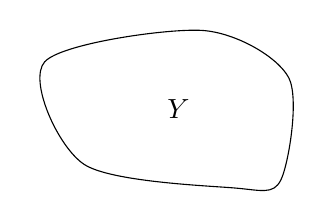
\begin{tikzpicture}
      \draw plot [smooth cycle] coordinates {(-1.2, -0.7) (0.7, -1) (1.3, -0.9) (1.4, 0.4) (0.3, 1) (-1.7, 0.6)};

      \node {$Y$};
    \end{tikzpicture}
  \end{center}
  We put a billiard ball in $Y$ and set it in motion. We want to see if it has periodic orbits.

  Two subsequent collisions tend to look like this:
  \begin{center}
    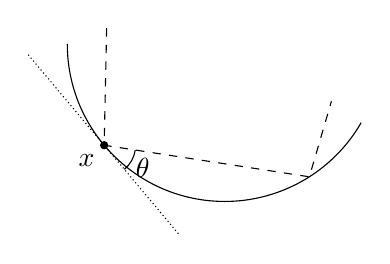
\begin{tikzpicture}
      \draw (-2, 0) arc (180:330:2);

      \draw [dashed] (-1.5, 0.2) -- (-1.532, -1.286) -- (1.074, -1.687) -- +(73.71:1);

      \node [circ] at (-1.532, -1.286) {};
      \node [anchor = north east] at (-1.532, -1.286) {$x$};

      \draw [densely dotted] (-1.532, -1.286) +(130:1.5) -- +(-50:1.5);

      \draw (-1.532, -1.286) +(-50:0.4) arc(-50:-8.76:0.4) node [pos=0.1, right] {$\theta$};
    \end{tikzpicture}
  \end{center}
  We can parametrize this collision as $(x, v = \cos \theta) \in \partial Y \times (-1, 1)$. We can think of this as the unit disk bundle of cotangent bundle on $X = \partial Y \cong S^1$ with canonical symplectic form $\d x \wedge \d v$, using a fixed parametrization $\chi: S^1 \cong \R/\Z \to X$. If $\varphi(x, v) = (y, w)$, then $v$ is the projection of the unit vector pointing from $x$ to $y$ onto the tangent line at $x$. Thus,
  \[
    v = \frac{\chi(y) - \chi(x)}{\|\chi(y) - \chi(x)\|} \cdot \left.\frac{\d \chi}{\d s}\right|_{s = x} = \frac{\partial}{\partial x} (-\|\chi(x) - \chi(y)\|),
  \]
  and a similar formula holds for $w$, using that the angle of incidence is equal to the angle of reflection. Thus, we know that
  \[
    f(x) = -\|\chi(x) - \chi(y)\|
  \]
  is a generating function for $\varphi$.
%
%  There is then a function $\varphi$ that sends $(x, v)$ to the coordinates of the next collision. We claim this is in fact a symplectomorphism, and to do so, we shall find a generating function for it.
%
%  Let $Y \subseteq \R^2$ be a bounded, convex region, thought of as a billiard table, and let $X = \partial Y \cong S^1$. Let $\chi: S^1 \cong \R/\Z \to \R^2$ be a parametrization of $X$.
%
%  The laws of physics determine a map $\varphi: X \times (-1, 1) \to X \times (-1, 1)$ as follows --- given $(x, \cos \theta)$, consider a billiard ball that leaves $X$ at an angle $\theta$ from the tangent. Then $\varphi(x, v) = (y, \cos \tau)$ is so that $y$ is the point where the ball first hits the boundary, and $\cos \tau$ is the angle at which the ball leaves after bouncing off.
%
%  We can think of $X \times (-1, 1)$ as the unit ball in the cotangent, and $\omega = \d x \wedge \d v$ is the canonical symplectic form. We claim that $\varphi$ is area preserving. To show this, we find a generating function $f$ for $\varphi$. We define $f: X \times X \to \R$ by
%  \[
%    f(x, y) = - \|\chi(x) - \chi(y)\|.
%  \]
%  This is smooth off the diagonal, and we have
%  \begin{align*}
%    \frac{\partial f}{\partial x}(x, y) &= \frac{\chi(y) - \chi(x)}{\|\chi(y) - \chi(x)\|} \cdot \left. \frac{\d \chi}{\d s} \right|_{s = x} = \cos \theta = v\\
%    \frac{\partial f}{\partial y}(x, y) &= \frac{\chi(x) - \chi(y)}{\|\chi(y) - \chi(x)\|} \cdot \left. \frac{\d \chi}{\d s} \right|_{s = y} = - \cos \nu = -w.
%  \end{align*}
%  So $f$ is indeed a generating function for $\varphi$.

  The conclusion is that the $N$-periodic points are given by the critical points of
  \[
    (x_1, \ldots, x_N) \mapsto - |\chi(x_1) - \chi(x_2)| - |\chi(x_2) - \chi(x_3)| - \cdots - |\chi(x_N) - \chi(x_1)|.
  \]
  Up to a sign, this is the length of the ``generalized polygon'' with vertices $(x_1, \ldots, x_N)$.
\end{eg}

In general, if $X$ is a compact manifold, and $\varphi: T^*X \to T^*X$ is a symplectomorphism generated by a function $f$, then the number of fixed points of $\varphi$ are the number of fixed points of $\psi(x) = f(x, x)$. By compactness, there is at least a minimum and a maximum, so $\varphi$ has at least two fixed points.

In fact,
\begin{thm}[Poincar\'e's last geometric theorem (Birkhoff, 1925)]\index{Poincar\'e's last geometric theorem}
  Let $\varphi: A \to A$ be an area-preserving diffeomorphism such that $\varphi$ preserves the boundary components, and twists them in opposite directions. Then $\varphi$ has at least two fixed points.
\end{thm}

\subsection{Lagrangian submanifolds and fixed points}
Recall what we have got so far. Let $(M, \omega)$ be a symplectic manifold, $\varphi: M \to M$. Then the graph of $\varphi$ is a subset of $M \times M$. Again let $\tilde{\omega}$ be the twisted product form on $M \times M$. Then we saw that a morphism $\varphi: M \to M$ is a symplectomorphism iff the graph of $\varphi$ is Lagrangian in $(M \times M, \tilde{\omega})$. Moreover, the set of fixed points is exactly $\Delta \cap \grph \varphi$, where $\Delta = \grph \id_M$ is the diagonal.

If $\varphi$ is ``close to'' the identity, map, then its graph is close to $\Delta$. Thus, we are naturally led to understanding the neighbourhoods of the identity. An important theorem is the following symplectic version of the tubular neighbourhood theorem:

\begin{thm}[Lagrangian neighbourhood theorem]\index{Lagrangian neighbourhood theorem}
  Let $(M, \omega)$ be a symplectic manifold, $X$ a compact Lagrangian submanifold, and $\omega_0$ the canonical symplectic form on $T^* X$. Then there exists neighbourhoods $U_0$ of $X$ in $T^* X$ and $U$ of $X$ in $M$ and a symplectomorphism $\varphi: \mathcal{U}_0 \to \mathcal{U}$ sending $X$ to $X$.
\end{thm}

An equivalent theorem is the following:
\begin{thm}[Weinstein]
  Let $M$ be a $2n$-dimensional manifold, $X$ $n$-dimensional compact submanifold, and $i: X \hookrightarrow M$ the inclusion, and symplectic forms $\omega_0, \omega_1$ on $M$ such that $i^* \omega_0 = i^* \omega_1 = 0$, i.e.\ $X$ is Lagrangian with respect to both symplectic structures. Then there exists neighbourhoods $\mathcal{U}_0, \mathcal{U}_1$ of $X$ in $M$ such that $\rho|_X = \id_X $ and $\rho^* \omega_1 = \omega_0$.
\end{thm}

We first prove these are equivalent. This amounts to identifying the (dual of the) cotangent bundle of $X$ with the normal bundle of $X$.

\begin{proof}[Proof of equivalence]
  If $(V, \Omega)$ is a symplectic vector space, $L$ a Lagrangian subspace, the bilinear form
  \begin{align*}
    \Omega: V/L \times L &\to \R\\
    ([v], u) &\to \Omega(v, u).
  \end{align*}
  is non-degenerate and gives a natural isomorphism $V/L \cong L^*$. Taking $V = T_p M$ and $L = T_p X$, we get an isomorphism
  \[
    NX = TM|_X /TX \cong T^* X.
  \]
  Thus, by the standard tubular neighbourhood theorem, there is a neighbourhood $\mathcal{N}_0$ of $X$ in $NX$ and a neighbourhood $\mathcal{N}$ of $X$ in $M$, and a diffeomorphism $\psi: \mathcal{N}_0 \to \mathcal{N}$. We now have two symplectic forms on $\mathcal{N}_0$ --- the one from the cotangent bundle and the pullback of that from $M$. Then applying the second theorem gives the first.

  Conversely, if we know the first theorem, then applying this twice gives us symplectomorphisms between neighbourhoods of $X$ in $M$ under each symplectic structure with a neighbourhood in the cotangent bundle.
\end{proof}

It now remains to prove the second theorem. This is essentially an application of the relative Moser theorem, which is where the magic happens. The bulk of the proof is to get ourselves into a situation where relative Moser applies.
\begin{proof}[Proof of second theorem]
  For $p \in X$, we define $V = T_p M$ and $U = T_p X$, and $W$ any complement of $U$. By assumption, $U$ is a Lagrangian subspace of both $(V, \omega_0|_p = \Omega_0)$ and $(V, \omega_1|_p = \Omega_1)$. We apply the following linear-algebraic lemma:

  \begin{lemma}
    Let $V$ be a $2n$-dimensional vector space, $\Omega_0, \Omega_1$ symplectic structures on $V$. Suppose $U$ is a subspace of $V$ Lagrangian with respect to both $\Omega_0$ and $\Omega_1$, and $W$ is any complement of $V$. Then we can construct canonically a linear isomorphism $H: V \to V$ such that $H|_U = \id_U$ and $H^* \Omega_1 = \Omega_2$.

    Note that the statement of the theorem doesn't mention $W$, but the construction of $H$ requires a complement of $V$, so it is canonical only after we pick a $W$. % prove lemma
  \end{lemma}
  By this lemma, we get canonically an isomorphism $H_p: T_p M \to T_p M$ such that $H_p|_{T_p X} = \id_{T_p X}$ and $H_p^* \omega_1|_p = \omega_0|_p$. The canonicity implies $H_p$ varies smoothly with $p$. We now apply the Whitney extension theorem
  \begin{thm}[Whitney extension theorem]\index{Whitney extension theorem}
    Let $X$ be a submanifold of $M$, $H_p: T_p M \to T_p M$ smooth family of isomorphisms such that $H_p|_{T_p X} = \id_{T_p X}$. Then there exists an neighbourhood $\mathcal{N}$ of $X$ in $M$ and an embedding $h: \mathcal{N} \to M$ such that $h|_X = \id_X$ and for all $p \in X$, $\d h_p = H_p$.
  \end{thm}
  So at $p \in X$, we have $h^* \omega_1|_p = (\d h_p)^*\omega_1|_P = h_p^* \omega_1|_p = \omega_0|_p$. So we are done by relative Moser.
\end{proof}

%\begin{proof}[Proof sketch of lemma]
%  We first claim that for $V$ a vector space, $\Omega$ a symplectic form, $U$ a Lagrangian subspace and $W$ any complement of $U$, there is a canonical way to convert $W$ into a Lagrangian complement of $V$, by taking the linear map $A: W \to U$ such that $\Omega(A\omega, \ph) = - \frac{1}{2} \Omega(w, \ph)$, and then taking % this might be wrong
%  \[
%    W' = (I - A) W.
%  \]
%  Thus in the situation of the lemma, we get two complements $W_0, W_1$ of $V$ that are Lagrangian with respect to $\Omega_0$ and $\Omega_1$ respectively. We set
%  \[
%    H = \id_U \oplus B: V \oplus W_0 \to U \oplus W_1,
%  \]
%  where $B$ satisfies $\Omega_0(w, u) = \Omega_1(Bw, u)$. Then $H^* \Omega_1 = \Omega_0$.
%\end{proof}

\begin{eg}
  We can use this result to understand the neighbourhood of the identity in the group $\Symp(M, \omega)$ of symplectomorphisms of a symplectic manifold $(M, \omega)$.

  Suppose $\varphi, \id \in \Symp(M, \omega)$. Then the graphs $\Gamma_\varphi$ and $\Delta = \Gamma_{\id}$ are Lagrangian submanifolds of $(M \times M, \tilde{\omega})$. Then by our theorem, there is a neighbourhood $\mathcal{U}$ of $\Delta$ in $(M \times M, \tilde{\omega})$ that is symplectomorphic to a neighbourhood $\mathcal{U}_0$ of the zero section of $(T^*M, \omega_0)$.

  Suppose $\varphi$ is sufficiently $C^0$-close to $\id$. Then $\Gamma_\varphi \subseteq \mathcal{U}$. If $\varphi$ is sufficiently $C^1$-close to the identity, then the image of $\Gamma_\varphi$ in $\mathcal{U}_0$ is a smooth section $X_\mu$ for some $1$-form $\mu$.

  Now $\varphi$ is a symplectomorphism iff $\Gamma_\varphi$ is Lagrangian iff $X_\mu$ is Lagrangian iff $\mu$ is closed. So a small $C^1$-neighbourhood of $\id$ in $\Sym(M, \omega)$ is ``the same as'' a small $C^1$-neighbourhood of the zero-section in the space of closed $1$-forms on $X$.
\end{eg}

We can also use this to understand fixed points of symplectomorphisms (again!).
\begin{thm}
  Let $(M, \omega)$ be a compact symplectic manifold such that $H^1_{\dR}(M) = 0$. Then any symplectomorphism $\varphi: M \to M$ sufficiently close to the identity has at least two fixed points.
\end{thm}

\begin{proof}
  The graph of $\varphi$ corresponds to a closed $1$-form on $M$. Since $\mu$ is closed and $H^1_{\dR}(M) = 0$, we know $\mu = \d h$ for some $h \in C^\infty$. Since $M$ is compact, $h$ has at least two critical points (the global maximum and minimum). Since the fixed points corresponding to the points where $\mu$ vanish (so that $\Gamma_\varphi$ intersects $\Delta$), we are done.
\end{proof}
Counting fixed points of symplectomorphisms is a rather popular topic in symplectic geometry, and Arnold made some conjectures about these. A version of this is
\begin{thm}[Arnold conjecture] % check
  Let $(M, \omega)$ be a compact symplectic manifold of dimension $2n$, and $\varphi: M \to M$ a symplectomorphism. Suppose $\varphi$ is \emph{exactly homotopic} to the identity and \emph{non-degenerate}. Then the number of fixed points of $\varphi$ is at least $\sum_{i = 0}^{2n} \dim H^i(M, \R)$.
\end{thm}
We should think of the sum $\sum_{i = 0}^{2n} \dim H^i(M, \R)$ as the minimal number of critical points of a function, as Morse theory tells us.

We ought to define the words we used in the theorem:

\begin{defi}[Exactly homotopic]\index{exactly homotopic}
  We say $\varphi$ is \emph{exactly homotopic} to the identity if there is isotopy $\rho_t: M \to M$ such that $\rho_0 = \id$ and $\rho_1 = \varphi$, and further there is some $1$-periodic family of functions $h_t$ such that $\rho_t$ is generated by the vector field $v_t$ defined by $\iota_{v_t}^* \omega = \d h_t$.
\end{defi}
The condition $\iota_{v_t}^* \omega \d h_t$ says $v_t$ is a Hamiltonian vector field, which we will discuss soon after this.

\begin{defi}[Non-degenerate function]\index{non-degenerate function}
  A endomorphism $\varphi: M \to M$ is non-degenerate iff all its fixed points are non-degenerate, i.e.\ if $p$ is a fixed point, then $\det (\id - \d \varphi_p) \not= 0$.
\end{defi}
\begin{eg}
  In the original statement of the Arnold conjecture, which is the case $(T^2, \d \theta_1 \wedge \d \theta_2)$, any symplectomorphism has at least $4$ fixed points.
\end{eg}

In the case where $h_t$ is actually not time dependent, Arnold's conjecture is easy to prove.

\section{Complex structures}
\subsection{Almost complex structures}
Symplectic manifolds are very closely related to complex manifolds. A first (weak) hint of this fact is that they both have to be even dimensional! In general, symplectic manifolds will have \emph{almost} complex structures, but this need not actually come from a genuine complex structure. If it does, then we say it is \emph{K\"ahler}, which is a very strong structure on the manifold.

We begin by explaining what almost complex structures are, again starting from the linear algebraic side of the story. A complex vector space can be thought of as a real vector space with a linear endomorphism that acts as ``multiplication by $i$''.

\begin{defi}[Complex structure]\index{complex structure}
  Let $V$ be a vector space. A \emph{complex structure} is a linear $J: V \to V$ with $J^2 = -1$.
\end{defi}
Here we call it a complex structure. When we move on to manifolds, we will call this ``almost complex'', and a complex structure is a stronger condition. It is clear that

\begin{lemma}
  There is a correspondence between real vector spaces with a complex structure and complex vector spaces, where $J$ acts as multiplication by $i$.\fakeqed
\end{lemma}

Our symplectic manifolds come with symplectic forms on the tangent space. We require the following compatibility condition:

\begin{defi}[Compatible complex structure]\index{compatible complex structure}
  Let $(V, \Omega)$ be a symplectic vector space, and $J$ a complex structure on $V$. We say $J$ is \emph{compatible} with $\Omega$ if $G_J(u, v) = \Omega(u, Jv)$ is an inner product. In other words, we need
  \[
    \Omega(Ju, Jv) = \Omega(u, v),\quad \Omega(v, Jv) \geq 0
  \]
  with equality iff $v = 0$.
\end{defi}

\begin{eg}
  On the standard symplectic vector space $(\R^{2n}, \Omega)$, we set
  \[
    J_0(e_i) = f_i,\quad J_0(f_i) = - e_i.
  \]
  We can then check that this is compatible with the symplectic structure, and in fact gives the standard inner product.
\end{eg}

\begin{prop}[Polar decomposition]\index{polar decomposition}
  Let $(V, \Omega)$ be a symplectic vector space, and $G$ an inner product on $V$. Then from $G$, we can \emph{canonically} construct a compatible complex structure $J$ on $(V, \Omega)$. If $G = G_{J}$ for some $J$, then this process returns $J$.
\end{prop}

Note that in general, $G_J(u, v) = \Omega(u, Jv) \not= G(u, v)$.
\begin{proof}
  Since $\Omega, G$ are non-degenerate, we know
  \[
    \Omega(u, v) = G(u, Av)
  \]
  for some $A: V \to V$. If $A^2 = -1$, then we are done, and set $J = A$. In general, we also know that $A$ is skew-symmetric, i.e.\ $G(Au, v) = G(u, -Av)$, which is clear since $\Omega$ is anti-symmetric. Since $AA^t$ is symmetric and positive definite, it makes sense to write down $\sqrt{AA^T}$ (e.g.\ by diagonalizing), and we take
  \[
    J = \sqrt{AA^t}^{-1} A = \sqrt{-A^2}^{-1} A.
  \]
  It is clear that $J^2 = -1$, since $A$ commutes with $\sqrt{AA^t}$, so this is a complex structure. We can write this as $A = \sqrt{AA^T} J$, and this is called the \emph{(left)} \term{polar decomposition} of $A$.

  We now check that $J$ is a compatible, i.e.\ $G_J(u, v) = \Omega(u, Jv)$ is symmetric and positive definite. But
  \[
    G_J(u, v) = G(u, \sqrt{AA^t}v),
  \]
  and we are done since $\sqrt{AA^t}$ is positive and symmetric.
\end{proof}

\begin{notation}
  Let $(V, \Omega)$ be a symplectic vector space. We write \term{$\mathcal{J}(V, \Omega)$} for the space of all compatible complex structures on $(V, \Omega)$.
\end{notation}

\begin{prop}
  $\mathcal{J}(V, \Omega)$ is path-connected.
\end{prop}

\begin{proof}
  Let $J_0, J_1 \in \mathcal{J}(V, \Omega)$. Then this induces inner products $G_{J_0}, G_{J_1}$. Let $G_t = (1 - t) G_{J_0} + t G_{J_1}$ be a smooth family of inner products on $V$. Then apply polar decomposition to get a family of complex structures that start from $J_0$ to $J_1$.
\end{proof}
A quick adaptation of the proof shows it is in fact contractible.

We now move on to the case of manifolds.

\begin{defi}[Almost complex structure]\index{almost complex structure}
  An \emph{almost complex structure} $J$ on a manifold is a smooth field of complex structures on the tangent space $J_p: T_p M \to T_p M$, $J_p^2 = -1$.
\end{defi}

\begin{eg}
  Suppose $M$ is a complex manifold with local complex coordinates $z_1, \ldots, z_n$ on $U \subseteq M$. We have real coordinates $\{x_i, y_i\}$ given by
  \[
    z_i = x_i + i y_i.
  \]
  The tangent space is spanned by $\frac{\partial}{\partial x_i}, \frac{\partial }{\partial y_i}$. We define $J$ by
  \[
    J_p\left(\frac{\partial}{\partial x_j}\right) = \frac{\partial}{\partial y_j},\quad J_p\left(\frac{\partial}{\partial y_j}\right) = - \frac{\partial}{\partial x_j}.
  \]
  The Cauchy--Riemann equations imply this is globally well-defined. This $J$ is called the \term{canonical almost-complex structure} on the complex manifold $M$.
\end{eg}
\begin{defi}[Integrable almost complex structure]\index{integrable almost complex structures}\index{almost complex structure!integrable}
  An almost complex structure on $M$ is called \emph{integrable} if it is induced by a complex structure.
\end{defi}

\begin{eg}
  It is a fact that $\CP^2 \# \CP^2 \# \CP^2$ has an almost complex but no complex structure.
\end{eg}

\begin{defi}[Compatible almost complex structure]\index{compatible almost complex structure}\index{almost complex structure!compatible}
  An almost complex structure $J$ on $M$ is \emph{compatible} with a symplectic structure $\omega$ if $J_p$ is compatible with $\omega_p$ for all $p \in M$. In this case, $(\omega, g_J, J)$ is called a \emph{compatible triple}.
\end{defi}
Any two of the structures determine the three, and this gives rise to the nice fact that the intersection of any two of $O(2n)$, $\Sp(2n, \R)$ and $\GL(n, \C)$ is $\U(n)$.

Performing polar decomposition pointwise gives
\begin{prop}
  Let $(M, \omega)$ be a symplectic manifold, and $g$ a metric on $M$. Then from $g$ we can canonically construct a compatible almost complex structure $J$.\fakeqed
\end{prop}

As before, in general, $g_J(\ph, \ph)\not= g(\ph, \ph)$.

\begin{cor}
  Any symplectic manifold has a compatible almost complex structure.\fakeqed
\end{cor}

The converse does not hold. For example, $S^6$ is almost complex but not symplectic.

\begin{notation}
  Let $(M, \omega)$ be a symplectic manifold. We write \term{$\mathcal{J}(V, \Omega)$} for the space of all compatible almost complex structures on $(M, \omega)$.
\end{notation}
The same proof as before shows that
\begin{prop}
  $J(M, \omega)$ is contractible.\fakeqed
\end{prop}

\begin{prop}
  Let $J$ be an almost complex structure on $M$ that is compatible with $\omega_0$ and $\omega_1$. Then $\omega_0$ and $\omega_1$ are deformation equivalent.
\end{prop}

\begin{proof}
  Check that $\omega_t = (1 - t) \omega_0 + t \omega_1$ works, which is non-degenerate since $\omega_t(\ph, J\ph)$ is a positive linear combination of inner products, hence is non-degenerate.
\end{proof}

\begin{prop}
  Let $(M, \omega)$ be a symplectic manifold, $J$ a compatible almost complex structure. If $X$ is an almost complex submanifold of $(M, J)$, i.e.\ $J(TX) = TX$, then $X$ is a symplectic submanifold of $(M, \omega)$.
\end{prop}

\begin{proof}
  We only have to check $\omega|_{TX}$ is non-degenerate, but $\Omega(\ph, J\ph)$ is a metric, so is in particular non-degenerate.
\end{proof}

We shall not prove the following theorem:
\begin{thm}[Gromov]
  Let $(M, J)$ be an almost complex manifold with $M$ open, i.e.\ $M$ has no closed connected components. Then there exists a symplectic form $\omega$ in any even $2$-cohomology class and such that $J$ is homotopic to an almost complex structure compatible with $\omega$.\fakeqed
\end{thm}

\subsection{Dolbeault theory}
An almost complex structure on a manifold allows us to discuss the notion of holomorphicity, and this will in turn allow us to stratify our $k$-forms in terms of ``how holomorphic'' they are.

Let $(M, J)$ be an almost complex manifold. By complexifying $TM$ to $TM \otimes \C$ and then extending $J$ linearly, we can split $TM \otimes \C$ into its $\pm i$ eigenspace.
\begin{notation}
  We write \term{$T_{1, 0}$} for the $+i$ eigenspace of $J$ and \term{$T_{1, 0}$} for the $-i$-eigenspace of $J$. These are called the \term{$J$-holomorphic tangent vectors}\index{holomorphic tangent vector} and the \term{$J$-anti-holomorphic tangent vectors}\index{anti-holomorphic tangent vector} respectively.
\end{notation}
We write \term{$T_{1, 0}$} for the $+i$ eigenspace of $J$, and \term{$T_{0, 1}$} the $-i$-eigenspace of $J$. Then we have a splitting
\[
  TM \otimes \C \overset{\sim}{\to} T_{1, 0} \oplus T_{0, 1}.
\]
We can explicitly write down the projection maps as
\begin{align*}
  \pi_{1, 0} (w) &= \frac{1}{2} (w - i J w)\\
  \pi_{0, 1} (w) &= \frac{1}{2} (w + i J w).
\end{align*}
\begin{eg}
  On a complex manifold with local complex coordinates $(z_1, \ldots, z_n)$, the holomorphic tangent vectors $T_{1, 0}$ is spanned by the $\frac{\partial}{\partial z_j}$, while $T_{0, 1}$ is spanned by the $\frac{\partial}{\partial \bar{z}_j}$.
\end{eg}
Similarly, we can complexify the cotangent bundle, and considering the $\pm i$ eigenspaces of (the dual of) $J$ gives a splitting\index{$T^{1, 0}$}\index{$T^{0, 1}$}
\[
  (\pi^{1, 0}, \pi^{0, 1}): T^*M \otimes C \overset{\sim}{\to} T^{1, 0} \oplus T^{0, 1}.
\]
These are the \term{complex linear cotangent vectors} and \term{complex anti-linear cotangent vectors}.
\begin{eg}
  In the complex case, $T^{1, 0}$ is spanned by the $\d z_j$ and $T^{0, 1}$ is spanned by the $\d \bar{z}_j$.
\end{eg}

More generally, we can decompose\index{$\Lambda^{p, q}$}
\[
  \exterior^k (T^* M \otimes \C) = \exterior^k (T^{1, 0} \oplus T^{0, 1}) = \bigoplus_{p + q = k} \left(\exterior^\ell T^{1, 0}\right) \otimes \left(\exterior^m T^{0, 1}\right) \equiv \bigoplus_{p + q = k} \Lambda^{p, q}.
\]
We write\index{$\Omega^{p, q}$}\index{$\Omega^k(M, \C)$}
\begin{align*}
  \Omega^k (M, \C) &= \text{sections of }\Lambda^k (T^* M \otimes \C)\\
  \Omega^{p, q}(M, \C) &= \text{sections of }\Lambda^{p, q}.
\end{align*}
So
\[
  \Omega^k(M, \C) = \bigoplus_{p + q = k} \Omega^{p, q} (M, \C).
\]
The sections in $\Omega^{p, q}(M, \C)$ are called \term{forms of type $(p, q)$}.
\begin{eg}
  In the complex case, we have, locally,
  \[
    \Lambda^{p, q}_p = \C\{\d z_I \wedge \d z_K : |I| = \ell, |K| = m\}
  \]
  and
  \[
    \Omega^{p, q} = \left\{\sum_{|I| = p, |K| = q} b_{I, K}\; \d z_I \wedge \d \bar{z}_K : b_{IK} \in C^\infty(U, \C)\right\}.
  \]
\end{eg}

As always, we have projections
\[
  \pi^{p, q}: \exterior^k (T^*M \otimes \C ) \to \Lambda^{p, q}.
\]
Combining the exterior derivative $\d: \Omega^k(M, \C) \to \Omega^{k - 1}(M, \C)$ with projections yield the $\partial$ and $\bar{\partial}$ operators
\begin{align*}
  \partial: \Omega^{p, q} &\to \Omega^{p + 1, q}\\
  \bar{\partial}: \Omega^{p, q} &\to \Omega^{p, q + 1}.
\end{align*}
Observe that for functions $f$, we have $\d f = \partial f + \bar{\partial} f$, but this is not necessarily true in general.

\begin{defi}[$J$-holomorphic]\index{$J$-holomorphic}\index{$J$-anti-holomorphic}
  We say a function $f$ is \emph{$J$-holomorphic} if $\bar{\partial} f = 0$, and \emph{$J$-anti-holomorphic} if $\partial f = 0$.
\end{defi}

It would be very nice if the sequence
\[
  \begin{tikzcd}
    \Omega^{p, q} \ar[r, "\bar{\partial}"] &
    \Omega^{p, q + 1} \ar[r, "\bar{\partial}"] &
    \Omega^{p, q + 2} \ar[r, "\bar{\partial}"] &
    \cdots
  \end{tikzcd}
\]
were a chain complex, i.e.\ $\bar{\partial}^2 = 0$. This is not always true. However, this is true in the case where $J$ is integrable. Indeed, if $M$ is a complex manifold and $\beta \in \Omega^k(M, \C)$, then in local complex coordinates, we can write
\[
  \beta = \sum_{p + q = k} \left(\sum_{|I| = p, |K| = q} b_{I, K}\; \d z_I \wedge \d \bar{z}_K\right).
\]
So
\begin{align*}
  \d \beta &= \sum_{p + q = k} \left(\sum_{|I| = p, |K| = q} \d b_{I, K}\wedge \d z_I \wedge \d \bar{z}_K\right)\\
  &= \sum_{p + q = k} \left(\sum_{|I| = p, |K| = q} (\partial + \bar{\partial}) b_{I, K}\wedge \d z_I \wedge \d \bar{z}_K\right)\\
  &= (\partial + \bar{\partial}) \sum_{p + q = k} \left(\sum_{|I| = p, |K| = q} b_{I, K}\d z_I \wedge \d \bar{z}_K\right)
\end{align*}
Thus, on a complex manifold, $\d = \partial + \bar{\partial}$.

Thus, if $\beta \in \Omega^{p, q}$, then
\[
  0 = \d^2 \beta = \partial^2 \beta + (\partial \bar{\partial} + \bar{\partial} \partial) \beta + \bar{\partial}^2 \beta.
\]
Since the three terms are of different types, it follows that
\[
  \partial^2 = \bar{\partial}^2 = \partial\bar{\partial} + \bar{\partial}\partial = 0.
\]
In fact, the converse of this computation is also true, which we will not prove:
\begin{thm}[Newlander--Nirenberg]\index{Newlander--Nirenberg}
  The following are equivalent:
  \begin{multicols}{2}
    \begin{itemize}
      \item $\bar{\partial}^2 = 0$
      \item $\partial^2 = 0$
      \item $\d = \partial + \bar{\partial}$
      \item $J$ is integrable
      \item $\mathcal{N} = 0$
      \item[ ]
    \end{itemize}
  \end{multicols}
  where $\mathcal{N}$ is the \term{Nijenhuis torsion}
  \[
    \mathcal{N}(X, Y) = [JX, JY] - J[JX, Y] - J[X, JY] - [X, Y].\fakeqed
  \]
\end{thm}

When our manifold is complex, we can then consider the cohomology of the chain complex.
\begin{defi}[Dolbeault cohomology groups]
  Let $(M, J)$ be a manifold with an integrable almost complex structure. The \term{Dolbeault cohomology groups} are the cohomology groups of the cochain complex
  \[
    \begin{tikzcd}
      \Omega^{p, q} \ar[r, "\bar{\partial}"] &
      \Omega^{p, q + 1} \ar[r, "\bar{\partial}"] &
      \Omega^{p, q + 2} \ar[r, "\bar{\partial}"] &
      \cdots
    \end{tikzcd}.
  \]
  Explicitly,
  \[
    H^{p, q}_{\Dolb} (M) = \frac{\ker(\bar{\partial}: \Omega^{p, q} \to \Omega^{p, q + 1})}{\im (\bar{\partial}: \Omega^{p, q - 1} \to \Omega^{p, q})}.
  \]
\end{defi}

\subsection{\tph{K\"ahler}{K\"ahler}{K&auml;hler} manifolds}
In the best possible scenario, we would have a symplectic manifold with a compatible, integrable almost complex structure. Such manifolds are called \emph{K\"ahler} manifolds.
\begin{defi}[K\"ahler manifold]\index{K\"ahler manifold}
  A \emph{K\"ahler manifold} is a symplectic manifold equipped with a compatible integrable almost complex structure. Then $\omega$ is called a \term{K\"ahler form}.
\end{defi}

Let $(M, \omega, J)$ be a K\"ahler manifold. What can we say about the K\"ahler form $\omega$? We can decompose it as
\[
  \omega \in \Omega^2(M) \subseteq \Omega^2(M, \C) = \Omega^{2, 0} \oplus \Omega^{1, 1} \oplus \Omega^{2, 2}.
\]
We claim that
\begin{lemma}
  $\omega \in \Omega^{1, 1}$.
\end{lemma}

\begin{proof}
  Since $\omega(\ph, J\ph)$ is symmetric, we have
  \[
    J^*\omega (u, v) = \omega(Ju, Jv) = \omega(v, JJu) = -\omega(v, -u) = \omega(u, v).
  \]
  So $J^* \omega = \omega$.

  On the other hand, $J^*$ acts on holomorphic forms as multiplication by $i$ and anti-holomorphic forms by multiplication by $-1$ (by definition). So it acts on $\Omega^{2, 0}$ and $\Omega^{0, 2}$ by multiplication by $-1$ (locally $\Omega^{2, 0}$ is spanned by $\d z_i \wedge \d z_j$, etc.), while it fixes $\Omega^{1, 1}$. So $\omega$ must lie in $\Omega^{1, 1}$.
\end{proof}
%Since $(M, J)$ is a complex manifold, we have the Dolbeault cohomology groups $H^{\ell, m}_{\Dolb}$. We can write our symplectic form as
%\[
%  \omega \in \Omega^2(M) \subseteq \Omega^2(M, \C) = \Omega^{2, 0} \oplus \Omega^{1, 1} \oplus \Omega^{0, 2}.
%\]
%On a complex chart $(U, z_1, \ldots, z_n)$, we can write
%\[
%  \omega = \sum_{j < k} a_{jk} \;\d z_j \wedge \d z_k + \sum_{j, k} + b_{jk} \d z_j \wedge \d \bar{z}_j + \sum_{j < k} c_{jk} \d \bar{z}_j \wedge \d \bar{z}_k.
%\]
%The compatibility condition implies $\omega(\ph, J\ph)$ is symmetric. We then have
%\[
%  J^* \omega(u, v) = \omega(Ju, Jv) = \omega(v, JJu) = - \omega(v, -u) = \omega(u, v).
%\]
%So $J^* \omega = \omega$. now observe that
%\[
%  J^* \d z_j = \d z_j \circ J = i \d z_j,\quad J^* \d \bar{z}_k = - i \d \bar{z}_k.
%\]
%Then
%\[
%  J^* \omega = \sum_{j < k}(-1) a_{jk}\; \d z_j \wedge \d z_k + \sum_{j, k} b_{jk}\; \d z_j \wedge \d \bar{z}_k + \sum_{j < k} (-1) c_{jk} \;\d \bar{z}_j \wedge \d \bar{z}_k.
%\]
%Then $J^* \omega = \omega$ implies $a_{jk} = c_{jk} = 0$. So we know that $\omega \in \Omega^{1, 1}$.

We can explore what the other conditions on $\omega$ tell us. Closedness implies
\[
  0 = \d \omega = \partial \omega + \bar{\partial} \omega = 0.
\]
So we have $\partial \omega = \bar{\partial} \omega = 0$. So in particular $\omega \in H^{1, 1}_{\Dolb}(M)$.

In local coordinates, we can write
\[
  \omega = \frac{i}{2} \sum_{j, k} h_{j, k} \;\d z_j \wedge \d \bar{z}_k
\]
for some $h_{j, k}$. The fact that $\omega$ is real valued, so that $\bar{\omega} = \omega$ gives some constraints on what the $h_{j k}$ can be. We compute
\[
  \bar{\omega} = -\frac{i}{2} \sum_{j, k}\overline{h_{jk}}\; \d \bar{z}_j \wedge \d z_k = \frac{i}{2} \sum_{j, k} \overline{h_{jk}} \;\d z_k \wedge \bar{z}_j.
\]
So we have
\[
  \overline{h}_{kj} = h_{jk}.
\]

The non-degeneracy condition $\omega^{\wedge n} \not= 0$ is equivalent to $\det h_{jk} \not= 0$, since
\[
  \omega^n = \left(\frac{i}{2}\right)^n n! \det(h_{jk}) \;\d z_1 \wedge \d \bar{z}_1 \wedge \cdots \wedge \d z_n \wedge \d \bar{z}_n.
\]
So $h_{jk}$ is a non-singular Hermitian matrix.

Finally, we take into account the compatibility condition $\omega(v, Jv) > 0$. If we write
\[
  v = \sum_j a_j \frac{\partial}{\partial z_j} + b_j \frac{\partial}{\partial \bar{z}_j},
\]
then we have
\[
  Jv = i \left(\sum_j a_j \frac{\partial}{\partial z_j} - b_j \frac{\partial}{\partial \bar{z}_j}\right).
\]
So we have
\[
  \omega(v, Jv) = \frac{i}{2} \sum h_{jk} (-ia_j b_k - ia_j b_k) = \sum h_{jk} a_j b_k > 0.
\]
So the conclusion is that $h_{jk}$ is positive definite.

Thus, the conclusion is
\begin{thm}
  A K\"ahler form $\omega$ on a complex manifold $M$ is a $\partial$- and $\bar{\partial}$-closed form of type $(1, 1)$ which on a local chart is given by
  \[
    \omega = \frac{i}{2} \sum_{j, k} h_{jk} \;\d z_j \wedge \d \bar{z}_k
  \]
  where at each point, the matrix $(h_{jk})$ is Hermitian and positive definite.
\end{thm}

Often, we start with a complex manifold, and want to show that it has a K\"ahler form. How can we do so? First observe that we have the following proposition:
\begin{prop}
  Let $(M, \omega)$ be a complex K\"ahler manifold. If $X \subseteq M$ is a complex submanifold, then $(X, i^* \omega)$ is K\"ahler, and this is called a \term{K\"ahler submanifold}.\fakeqed
\end{prop}

In particular, if we can construct K\"ahler forms on $\C^n$ and $\CP^n$, then we have K\"ahler forms for a lot of our favorite complex manifolds, and in particular complex projective varieties.

But we still have to construct some K\"ahler forms to begin with. To do so, we use so-called \emph{strictly plurisubharmonic functions}.
\begin{defi}[Strictly plurisubharmonic (spsh)]\index{strictly plurisubharmonic}\index{spsh}
  A function $\rho \in C^\infty(M, \R)$ is strictly plurisubharmonic (spsh) if locally, $\left(\frac{\partial^2 \rho}{\partial z_j \partial \bar{z}_k}\right)$ is positive definite.
\end{defi}
\begin{prop}
  Let $M$ be a complex manifold, and $\rho \in C^\infty(M; \R)$ strictly plurisubharmonic. Then
  \[
    \omega = \frac{i}{2} \partial \bar{\partial} \rho
  \]
  is a K\"ahler form.
\end{prop}
We call $\rho$ the \term{K\"ahler potential} for $\omega$.
\begin{proof}
  $\omega$ is indeed a $2$-form of type (1, 1). Since $\partial^2 = \bar{\partial}^2 = 0$ and $\partial \bar{\partial} = -\bar{\partial} \partial$, we know $\partial \omega = \bar{\partial} \omega = 0$. We also have
  \[
    \omega = \frac{i}{2} \sum_{j, k} \frac{\partial^2 \rho}{\partial z_j \partial \bar{z}_k}\;\d z_j\wedge \d \bar{z}_k,
  \]
  and the matrix is Hermitian positive definite by assumption.
\end{proof}

\begin{eg}
  If $M = \C^n \cong \R^{2n}$, we take
  \[
    \rho(\mathbf{z}) = |\mathbf{z}|^2 = \sum z_k \bar{z}_k.
  \]
  Then we have
  \[
    h_{jk} = \frac{\partial^2 \rho}{\partial z_j \partial \bar{z}_k} = \delta_{jk},
  \]
  so this is strictly plurisubharmonic. Then
  \begin{align*}
    \omega &= \frac{i}{2} \sum \d z_j \wedge \d \bar{z}_k \\
    &= \frac{i}{2} \sum \d (x_j + i y_j) \wedge \d (x_k - i y_k)\\
    &= \sum \d x_k \wedge \d y_k,
  \end{align*}
  which is the standard symplectic form. So $(\C^n, \omega)$ is K\"ahler and $\rho = |z|^2$ is a (global) K\"ahler potential for $\omega_0$.
\end{eg}

There is a local converse to this result.

\begin{prop}
  Let $M$ be a complex manifold, $\omega$ a closed real-valued $(1, 1)$-form and $p \in M$, then there exists a neighbourhood $U$ of $p$ in $M$ and a $\rho \in C^\infty(U, \R)$ such that
  \[
    \omega = i \partial \bar{\partial} \rho\text{ on }U.
  \]
\end{prop}

\begin{proof}
  This uses the holomorphic version of the Poincar\'e lemma.
\end{proof}

When $\rho$ is K\"ahler, such a $\rho$ is called a \term{local K\"ahler potential} for $\omega$.

Note that it is not possible to have a global K\"ahler potential on a closed K\"ahler manifold, because if $\omega = \frac{i}{2}\partial \bar{\partial} \rho$, then
\[
  \omega = \d \left(\frac{i}{2} \bar{\partial} \rho\right)
\]
is exact, and we know symplectic forms cannot be exact.

\begin{eg}
  Let $M = \C^n$ and
  \[
    \rho(z) = \log (|z|^2 + 1).
  \]
  It is an exercise to check that $\rho$ is strictly plurisubharmonic. Then
  \[
    \omega_{FS} = \frac{i}{2} \partial \bar{\partial} (\log(|z^2| + 1))
  \]
  is another K\"ahler form on $\C^n$, called the \term{Fubini--Study form}.
\end{eg}
The reason this is interesting is that it allows us to put a K\"ahler structure on $\CP^n$.
\begin{eg}
  Let $M = \CP^n$. Using homogeneous coordinates, this is covered by the open sets
  \[
    U_j = \{[z_0, \ldots, z_n] \in \CP^n \mid z_j \not= 0\}.
  \]
  with the chart given by
  \begin{align*}
    \varphi_j: U_j &\to \C^n\\
    [z_0, \ldots, z_n] &\mapsto \left(\frac{z_0}{z_j}, \ldots, \frac{z_{j - 1}}{z_j}, \frac{z_{j + 1}}{z_j}, \ldots, \frac{z_n}{z_j}\right).
  \end{align*}
  One can check that $\varphi_j^* \omega_{FS} = \varphi_k^* \omega_{FS}$. Thus, these glue to give the \term{Fubini--Study form} on $\CP^n$, making it a K\"ahler manifold.
\end{eg}

\subsection{Hodge theory}
So what we have got so far is that if we have a complex manifold, then we can decompose
\[
  \Omega^k(M; \C) = \bigoplus_{p + q = k} \Omega^{p, q},
\]
and using $\bar{\partial}: \Omega^{p, q} \to \Omega^{p, q + 1}$, we defined the Dolbeault cohomology groups
\[
  H_{\Dolb}^{p, q}(M) = \frac{\ker \bar{\partial}}{\im \bar{\partial}}.
\]
It would be nice if we also had a decomposition
\[
  H^k_{\dR} \cong \bigoplus_{p + q = k} H^{p, q}_{\Dolb}(M).
\]
This is not always true. However, it is true for compact K\"ahler manifolds:
\begin{thm}[Hodge decomposition theorem]\index{Hodge decomposition theorem}
  Let $(M, \omega)$ be a compact K\"haler manifold. Then
  \[
    H^k_{\dR} \cong \bigoplus_{p + q = k} H^{p, q}_{\Dolb}(M).
  \]
\end{thm}
To prove the theorem, we will first need a ``real'' analogue of the theorem. This is an analytic theorem that lets us find canonical representatives for each cohomology class. We can develop the same theory for Dolbeault cohomology, and see that the canonical representatives for Dolbeault cohomology are the same as those for de Rham cohomology. We will not prove the analytic theorems, but just say how these things piece together.
\subsubsection*{Real Hodge theory}
Let $V$ be a real oriented vector space $m$ with inner product $G$. Then this induces an inner product on each $\Lambda^k = \exterior^k (V)$, denoted $\bra \ph, \ph\ket$, defined by
\[
  \bra v_1 \wedge \cdots \wedge v_k, w_1 \wedge \cdots \wedge w_k\ket = \det (G(v_i, w_j))_{i, j}
\]
Let $e_1, \ldots, e_n$ be an oriented orthonormal basis for $V$. Then
\[
  \{e_{j_1} \wedge \cdots \wedge e_{j_k} : 1 \leq j_1 < \cdots < j_k \leq m\}
\]
is an orthonormal basis for $\Lambda^k$.

\begin{defi}[Hodge star]\index{hodge star}
  The Hodge $*$-operator \index{$*$}$*: \Lambda^k \to \Lambda^{m - k}$ is defined by the relation
  \[
    \alpha \wedge *\beta = \bra \alpha, \beta\ket\; e_1 \wedge \cdots \wedge e_m.
  \]
\end{defi}
It is easy to see that the Hodge star is in fact an isomorphism. It is also not hard to verify the following properties:
\begin{prop}\leavevmode
  \begin{itemize}
    \item $*(e_1 \wedge \cdots \wedge e_k) = e_{k + 1} \wedge \cdots \wedge e_m$
    \item $*(e_{k + 1} \wedge \cdots \wedge e_m) = (-1)^{k(m - k)} e_1 \wedge \cdots \wedge e_k$.
    \item $** =\alpha = (-1)^{k(m - k)}\alpha$ for $\alpha \in \Lambda^k$.\fakeqed
  \end{itemize}
\end{prop}

In general, let $(M, g)$ be a compact real oriented Riemannian manifold of dimension $m$. Then $g$ gives an isomorphism $TM \cong T^*M$, and induces an inner product on each $T_p^* M$, which we will still denote $g_p$. This induces an inner product on each $\exterior^k T_p^*M$, which we will denote $\bra \ph, \ph \ket$ again.

The Riemannian metric and orientation gives us a volume form $\Vol \in \Omega^m(M)$, defined locally by
\[
  \Vol_p(e_1 \wedge \cdots \wedge e_m),
\]
where $e_1, \ldots, e_m$ is an oriented basis of $T_p^*M$. This induces an $L^2$-inner product on $\Omega^k(M)$,
\[
  \bra \alpha, \beta\ket_{L^2} = \int_M \bra \alpha, \beta\ket\;\Vol.
\]
Now apply Hodge $*$-operator to each $(V, G) = (T_p^* M, g_p)$ and $p \in M$. We then get
\begin{defi}[Hodge star operator]\index{Hodge star}\index{$*$}
  The \emph{Hodge $*$-operator} on forms $*: \Omega^k(M) \to \Omega^{m - k}(M)$ is defined by the equation
  \[
    \alpha \wedge (*\beta) = \bra \alpha ,\beta\ket \; \Vol.
  \]
\end{defi}

We again have some immediate properties.
\begin{prop}\leavevmode
  \begin{enumerate}
    \item $**\alpha = (-1)^{k(m - k)} \alpha$ for $\alpha \in \Omega^k(M)$.
    \item $*1 = \Vol$\fakeqed
  \end{enumerate}
\end{prop}

We now introduce the codifferential operator
\begin{defi}[Codifferential operator]\index{codifferential operator}\index{$\delta$}
  We define the \emph{codifferential operator} $\delta: \Omega^k \to \Omega^{k - 1}$ to be the $L^2$-formal adjoint of $d$. In other words, we require
  \[
    \bra \d \alpha, \beta\ket_{L^2} = \bra \alpha, \delta \beta\ket_{L^2}
  \]
  for all $\alpha \in \Omega^k$ and $\beta \in \Omega^{k + 1}$.
\end{defi}
We immediately see that
\begin{prop}
  $\delta^2 = 0$.
\end{prop}

Using the Hodge star, there is a very explicit formula for the codifferential (which in particular shows that it exists).
\begin{prop}
  \[
    \delta = (-1)^{m(k + 1) + 1} {*\,\d\, *} : \Omega^k \to \Omega^{k - 1}.
  \]
\end{prop}

\begin{proof}
  \begin{align*}
    \bra \d \alpha, \beta \ket_{L^2} &= \int_M \d \alpha \wedge * \beta\\
    &= \int_M \d (\alpha \wedge *\beta) - (-1)^k \int_M \alpha \wedge \d (*\beta)\\
    &= (-1)^{k + 1} \int_M \alpha \wedge \d (*\beta)\tag{Stokes'}\\
    &= (-1)^{k + 1} \int_M (-1)^{(m - k)k} \alpha \wedge **\d (*\beta)\\
    &= (-1)^{k + 1 + (m - k)k} \int_M \bra \alpha, {*\ \d\,*}\beta\ket.\qedhere
  \end{align*}
\end{proof}

We can now define the Laplace--Beltrami operator
\begin{defi}[Laplace--Beltrami operator]\index{Laplace--Beltrami operator}\index{Laplacian}
  We define the \emph{Laplacian}, or the \emph{Laplace--Beltrami operator} to be
  \[
    \Delta = \d \delta + \delta \d: \Omega^k \to \Omega^k.
  \]
\end{defi}

\begin{eg}
  If $M = \R^m$ with the Euclidean inner product, and $f \in \Omega^0(M) = C^\infty(M)$, then
  \[
    \Delta f = - \sum_{i = 1}^n \frac{\partial^2 f}{\partial x_i^2}.
  \]
\end{eg}

It is an exercise to prove the following
\begin{prop}\leavevmode
  \begin{enumerate}
    \item $\Delta * = *\Delta: \Omega^k \to \Omega^{m - k}$
    \item $\Delta = (\d + \delta)^2$
    \item $\bra \Delta \alpha, \beta\ket_{L^2} = \bra \alpha, \Delta \beta\ket_{L^2}$.
    \item $\Delta \alpha = 0$ iff $\d \alpha = \delta \alpha = 0$.\fakeqed
  \end{enumerate}
\end{prop}
In particular, (iv) follows from the fact that
\[
  \bra \Delta \alpha, \alpha\ket = \bra \d \alpha, \d \alpha\ket + \bra \delta \alpha, \delta \alpha\ket = \|\d \alpha\|_{L^2}^2 + \|\delta \alpha\|_{L^2}^2.
\]
Similar to IA Vector Calculus, we can define
\begin{defi}[Harmonic form]\index{harmonic form}
  A form $\alpha$ is \emph{harmonic} if $\Delta \alpha = 0$. We write\index{$\mathcal{H}^k$}
  \[
    \mathcal{H}^k = \{\alpha \in \Omega^k(m) \mid \Delta \alpha = 0\}
  \]
  for the space of harmonic forms.
\end{defi}
Observe there is a natural map $\mathcal{H}^k \to H^k_{\dR}(M)$, sending $\alpha$ to $[\alpha]$. The main result is that
\begin{thm}[Hodge decomposition theorem]\index{Hodge decomposition theorem}
  Let $(M, g)$ be a compact oriented Riemannian manifold. Then every cohomology class in $H_{\dR}^k(M)$ has a unique harmonic representation, i.e.\ the natural map $\mathcal{H} ^k \to H_{\dR}^k(M)$ is an isomorphism.\qedhere
\end{thm}
We will not prove this.

\subsubsection*{Complex Hodge theory}
We now see what we can do for complex K\"ahler manifolds. First check that
\begin{prop}
  Let $M$ be a complex manifold, $\dim_\C M = n$ and $(M, \omega)$ K\"ahler. Then
  \begin{enumerate}
    \item $*: \Omega^{p, q} \to \Omega^{n - p, n - q}$.
    \item $\Delta: \Omega^{p, q} \to \Omega^{p, q}$.\fakeqed
  \end{enumerate}
\end{prop}

define the $L^2$-adjoints $\bar{\partial}^* = \pm *\bar{\partial}*$ and $\partial^* = -- * \partial *$ with the appropriate signs as before, and then
\[
  \d = \partial + \bar{\partial},\quad \delta = \partial^* + \bar{\partial}^*.
\]
We can then define
\begin{align*}
  \Delta_{\partial} &= \partial \partial^* + \partial^* \partial : \Omega^{p, q} \to \Omega^{p, q}\\
  \Delta_{\bar{\partial}} &= \bar{\partial} \bar{\partial}^* + \bar{\partial}^* \bar{\partial} : \Omega^{p, q} \to \Omega^{p, q}.
\end{align*}

\begin{prop}
  If our manifold is K\"ahler, then
  \[
    \Delta = 2 \Delta_\partial = 2 \Delta_{\bar{\partial}}.\fakeqed
  \]
\end{prop}
So if we have a harmonic form, then it is in fact $\partial$ and $\bar{\partial}$-harmonic, and in particular it is $\partial$ and $\bar{\partial}$-closed. This give us a \emph{Hodge decomposition}
\[
  \mathcal{H}^k_\C = \bigoplus_{p + q = k} \mathcal{H}^{p, q},
\]
where\index{$\mathcal{H}^{p, q}$}
\[
  \mathcal{H}^{p, q} = \{\alpha \in \Omega^{p, q}(M): \Delta \alpha = 0\}.
\]
\begin{thm}[Hodge decomposition theorem]\index{Hodge decomposition theorem}
  Let $(M, \omega)$ be a compact K\"ahler manifold. The natural map $\mathcal{H}^{p, q} \to H_{\Dolb}^{p, q}$ is an isomorphism. Hence
  \[
    H^k_{\dR} (M; \C) \cong \mathcal{H}^k_{\C} = \bigoplus_{p + q = k} \mathcal{H}^{p, q} \cong \bigoplus_{p + q = k} H_{\Dolb}^{p, q}(M).\fakeqed
  \]
\end{thm}

What are some topological consequences of this? Recall the \term{Betti numbers} are defined by
\[
  b_k = \dim_\R H^k_{\dR}(M) = \dim_\C H^k_{\dR}(M; \C).
\]
We can further define the \term{Hodge numbers}
\[
  h_{p, q} = \dim_\C H^{p, q}_{\Dolb}(M).
\]
Then the Hodge theorem says
\[
  b_k = \sum_{p + q = k} h_{p, q}.
\]
Moreover, since
\[
  H_{\Dolb}^{p, q}(M) = \overline{H_{\Dolb}^{q, p}(M)}.
\]
So we have \term{Hodge symmetry},
\[
  h_{p, q} = h_{q, p}.
\]
Moreover, the $*$ operator induces an isomorphism
\[
  H^{p, q}_{\Dolb} \cong H_{\Dolb}^{n - p, n - q}.
\]
So we have
\[
  h_{p, q} = h_{n - p, n - q}.
\]
There is called \term{central symmetry}, or \term{Serre duality}. Thus, we know that
\begin{cor}
  Odd Betti numbers are even.
\end{cor}

\begin{proof}
  \[
    b_{2k + 1} = \sum_{p + q = 2k + 1} h_{p, q} = 2 \left(\sum_{p = 0}^k h_{p, 2k + 1 - p}\right).\qedhere
  \]
\end{proof}

\begin{cor}
  $h_{1, 0} = h_{0, 1} = \frac{1}{2}b_1$ is a topological invariant.
\end{cor}

We have also previously seen that for a general compact K\"ahler manifold, we have
\begin{prop}
  Even Betti numbers are positive.
\end{prop}

Recall that we proved this by arguing that $[\omega^k] \not= 0 \in H^{2k}(M)$. In fact, $\omega^k \in H^{k, k}_{\Dolb}(M)$, and so
\begin{prop}
  $h_{k, k} \not= 0$.\fakeqed % insert proof
\end{prop}

We usually organize these $h_{p, q}$ in the form of a \term{Hodge diamond}, e.g.
\begin{center}
  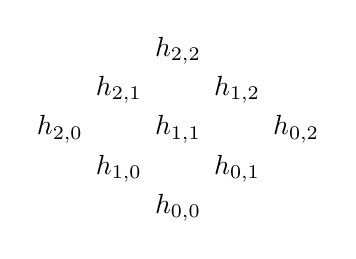
\begin{tikzpicture}[xscale=1.5, yscale=0.5]
    \node at (0, -2) {$h_{0, 0}$};
    \node at (-0.5, -1) {$h_{1, 0}$};
    \node at (0.5, -1) {$h_{0, 1}$};
    \node at (-1, 0) {$h_{2, 0}$};
    \node at (0, 0) {$h_{1, 1}$};
    \node at (1, 0) {$h_{0, 2}$};
    \node at (-0.5, 1) {$h_{2, 1}$};
    \node at (0.5, 1) {$h_{1, 2}$};
    \node at (0, 2) {$h_{2, 2}$};
  \end{tikzpicture}
\end{center}

%\subsection{Conclusion}
%So suppose $M$ is a compact manifold. When is there a symplectic manifold? Elementary necessary conditions involve
%\begin{itemize}
%  \item $M$ must be even-dimensional and orientable
%  \item There exists $[\omega] \in H^2(M)$ such that $[\omega^n] \not= 0$ by Stokes' theorem. Then $M$ must be almost complex.
%\end{itemize}
%
%For dimension $2$, being orientable implies K\"ahler.
%
%Note that $S^2$ is K\"ahler, and the only spheres that admit an almost complex structure are $S^2$ and $S^6$.
\section{Hamiltonian vector fields}
Symplectic geometry was first studied by physicists, who modeled their systems by a symplectic manifold. The \emph{Hamiltonian function} $H \in C^\infty(M)$, which returns the energy of a particular configuration, generates a vector field on $M$ which is the equation of motion of the system. In this chapter, we will discuss how this process works, and further study what happens when we have families of such Hamiltonian functions, giving rise to Lie group actions.

\subsection{Hamiltonian vector fields}
\begin{defi}[Hamiltonian vector field]\index{Hamiltonian vector field}
  Let $(M, \omega)$ be a symplectic manifold. If $H \in C^\infty(M)$, then since $\tilde{\omega}: TM \to T^*M$ is an isomorphism, there is a unique vector field $X_H$ on $M$ such that
  \[
    \iota_{X_H} \omega = \d H.
  \]
  We call $X_H$ the \emph{Hamiltonian vector field} with \term{Hamiltonian function} $H$.
\end{defi}

Suppose $X_H$ is complete (e.g.\ when $M$ is compact). This means we can integrate $X_H$, i.e.\ solve
\[
  \frac{\partial \rho_t}{\partial t} (p) = X_H(\rho_t(p)),\quad \rho_0(p) = p.
\]
These flow have some nice properties.
\begin{prop}
  If $X_H$ is a Hamiltonian vector field with flow $\rho_t$, then $\rho_t^* \omega = \omega$. In other words, each $\rho_t$ is a symplectomorphism.
\end{prop}

\begin{proof}
  It suffices to show that $\frac{\partial}{\partial t} \rho_t^* \omega = 0$. We have
  \[
    \frac{\d}{\d t} (\rho_t^* \omega) = \rho_t^* (\mathcal{L}_{X_H} \omega) = \rho_t^* (\d \iota_{X_H} \omega + \iota_{X_H} \d \omega) = \rho_t^* (\d \d H) = 0.\qedhere
  \]
\end{proof}

Thus, every function $H$ gives us a one-parameter subgroup of symplectomorphisms.

\begin{prop}
  $\rho_t$ preserves $H$, i.e.\ $\rho_t^* H = H$.
\end{prop}

\begin{proof}
  \[
    \frac{\d}{\d t} \rho_t^* H = \rho_t^* (\mathcal{L}_{X_H}H) = \rho_t^* (\iota_{X_H} \d H) = \rho_t^* (\iota_{X_H} \iota_{X_H}\omega) = 0.\qedhere
  \]
\end{proof}

So the flow lines of our vector field are contained in level sets of $H$.
\begin{eg}
  Take $(S^2, \omega = \d \theta \wedge \d h)$. Take
  \[
    H(h, \theta) = h
  \]
  to be the height function. Then $X_H$ solves
  \[
    \iota_{X_H} (\d \theta \wedge \d h) = \d h.
  \]
  So
  \[
    X_H = \frac{\partial}{\partial \theta},\quad \rho_t(h, \theta) = (h, \theta + t).
  \]
  As expected, the flow preserves height and the area form.
  \begin{center}
    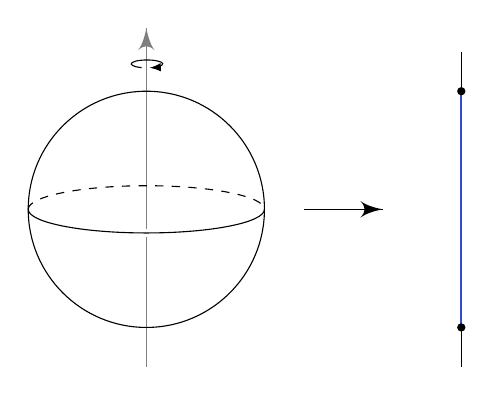
\begin{tikzpicture}
      \draw [->, gray] (0, -0.25) -- (0, 2.3);
      \draw [gray] (0, -2) -- (0, -0.35);

      \draw circle [radius=1.5];

      \draw [dashed] (-1.5, 0) arc(180:0:1.5 and 0.3);
      \draw (-1.5, 0) arc(180:360:1.5 and 0.3);

      \draw [-latex] (-0.06, 1.8) arc(250:-80:0.2 and 0.05);

      \draw [->] (2, 0) -- (3, 0);

      \draw (4, -2) -- (4, 2);
      \draw [mblue, thick] (4, -1.5) -- (4, 1.5);
      \node [circ] at (4, -1.5) {};
      \node [circ] at (4, 1.5) {};
    \end{tikzpicture}
  \end{center}
\end{eg}

We have seen that Hamiltonian vector fields are symplectic:
\begin{defi}[Symplectic vector field]\index{symplectic vector field}
  A vector field $X$ on $(M, \omega)$ is a \emph{symplectic vector field} if $\mathcal{L}_X \omega = 0$.
\end{defi}
Observe that
\[
  \mathcal{L}_X \omega= \iota_X \d \omega + \d \iota_X \omega = \d \iota_X \omega.
\]
So $X$ is symplectic iff $\iota_X \omega$ is closed, and is Hamiltonian if it is exact. Thus, locally, every symplectic vector field is Hamiltonian and globally, the obstruction lies in $H^1_{\dR}(M)$.

\begin{eg}
  Take $(T^2, \omega = \d \theta_1 \wedge \d \theta_2)$. Then $X_i = \frac{\partial}{\partial \theta_i}$ are symplectic but not Hamiltonian, since $\iota_{X_i} \omega = \d \theta_{2 - i}$ is closed but not exact.
\end{eg}

\begin{prop}
  Let $X, Y$ be symplectic vector fields on $(M, \omega)$. Then $[X, Y]$ is Hamiltonian.
\end{prop}
Recall that if $X, Y$ are vector fields on $M$ and $f \in C^\infty(M)$, then their \term{Lie bracket} is given by
\[
  [X, Y]f = (XY - YX)f.
\]
This makes $\chi(M)$, the space of vector fields on $M$, a Lie algebra.

In order to prove the proposition, we need the following identity:
\begin{ex}
  $\iota_{[X, Y]}\alpha = [\mathcal{L}_X, \iota_Y] \alpha = [\iota_X, \mathcal{L}_Y] \alpha$.
\end{ex}
%To prove this, check this on $0$-forms; exact $1$-forms; then check when both sides are anti-derivatives
%\[
%  \D (\alpha \wedge \beta) = \D \alpha \wedge \beta + (-1)^{\deg \alpha} \alpha \wedge \D \beta.
%\]

\begin{proof}[Proof of proposition]
  We need to check that $\iota_{[X, Y]} \omega$ is exact. By the exercise, this is
  \[
    \iota_{[X, Y]}\omega = \mathcal{L}_X \iota_Y \omega - \iota_Y \mathcal{L}_X \omega = \d (\iota_X \iota_Y \omega) + \iota_X \d \iota_Y \omega + \iota_Y \d \iota_X \omega - \iota_Y \iota_Y \d \omega.
  \]
  Since $X, Y$ are symplectic, we know $\d \iota_Y \omega = \d \iota_X \omega = 0$, and the last term always vanishes. So this is exact, and $\omega(Y, X)$ is a Hamiltonian function for $[X, Y]$.
\end{proof}

\begin{defi}[Poisson bracket]\index{Poisson bracket}
  Let $f, g \in C^\infty(M)$. We then define the \emph{Poisson bracket} $\{f, g\}$ by
  \[
    \{f, g\} = \omega(X_f, X_g).
  \]
\end{defi}
This is defined so that
\[
  X_{\{f, g\}} = -[X_f, X_g].
\]
\begin{ex}
  The Poisson bracket satisfies the Jacobi identity, and also the Leibniz rule
  \[
    \{f, gh\} = g\{f, h\} + \{f, g\}h.
  \]
\end{ex}
Thus, if $(M, \omega)$ is symplectic, then $(C^\infty(M), \{\ph, \ph\})$ is a \term{Poisson algebra}. This means it is a commutative, associative algebra with a Lie bracket that satisfies the Leibniz rule.

Further, the map $C^\infty(M) \to \chi(M)$ sending $H \mapsto X_H$ is a Lie algebra (anti-)homomorphism.

\begin{prop}
  $\{f, g\} = 0$ iff $f$ is constant along integral curves of $X_g$.
\end{prop}

\begin{proof}
  \[
    \mathcal{L}_{X_g} f = \iota_{X_g}\;\d f = \iota_{X_g} \iota_{X_f} \omega = \omega(X_f, X_g) = \{f, g\} = 0.\qedhere
  \]
\end{proof}

\begin{eg}
  If $M = \R^{2n}$ and $\omega = \omega_0 = \sum \d x_j \wedge \d y_j$, and $f \in C^\infty(\R^{2n})$, then
  \[
    X_f = \sum_i \left(\frac{\partial f}{\partial y_i} \frac{\partial}{\partial x_i} - \frac{\partial f}{\partial x_i} \frac{\partial }{\partial y_i}\right).
  \]
  If $\rho_0(p) = p$, then $\rho_t(p) = (x(t), y(t))$ is an integral curve for $X_f$ iff
  \[
    \frac{\d x_i}{\d t} = \frac{\partial f}{\partial y_i},\quad \frac{\partial y_i}{\partial t} = -\frac{\partial f}{\partial x_i}.
  \]
  In classical mechanics, these are known as \term{Hamilton equations}.
\end{eg}

\subsection{Integrable systems}
In classical mechanics, we usually have a fixed $H$, corresponding to the energy.
\begin{defi}[Hamiltonian system]\index{Hamiltonian system}
  A \emph{Hamiltonian system} is a triple $(M, \omega, H)$ where $(M, \omega)$ is a symplectic manifold and $H \in C^\infty(M)$, called the \term{Hamiltonian function}.
\end{defi}

\begin{defi}[Integral of motion]\index{integral of motion}
  A \emph{integral of motion}/\term{first integral}/\term{constant of motion}/\term{conserved quantity} of a Hamiltonian system is a function $f \in C^\infty(M)$ such that $\{f, H\} = 0$.
\end{defi}
For example, $H$ is an integral of motion. Are there others? Of course, we can write down $2H, H^2, H^{12}, e^H$, etc., but these are more-or-less the same as $H$.
\begin{defi}[Independent integrals of motion]\index{independent integrals of motion}
  We say $f_1, \ldots, f_n \in C^\infty(M)$ are \emph{independent} if $(\d f_1)_p, \ldots, (\d f_n)_p$ are linearly independent at all points on some dense subset of $M$.
\end{defi}

\begin{defi}[Commuting integrals of motion]\index{commuting integrals of motion}
  We say $f_1, \ldots, f_n \in C^\infty$ \emph{commute} if $\{f_i, f_j\} = 0$.
\end{defi}

If we have $n$ independent integrals of motion, then we clearly have $\dim M \geq n$. In fact, the commuting condition implies:
\begin{ex}
  Let $f_1, \ldots, f_n$ be independent commuting functions on $(M, \omega)$. Then $\dim M \geq 2n$.
\end{ex}
The idea is that the $(\d f_i)_p$ are not only independent, but span an isotropic subspace of $TM$.

If we have the maximum possible number of independent commuting first integrals, then we say we are integrable.
\begin{defi}[Completely integrable system]\index{completely integrable system}
  A Hamiltonian system $(M, \omega, H)$ of dimension $\dim M = 2n$ is \emph{(completely) integrable} if it has $n$ independent commuting integrals of motion $f_1 = H, f_2, \ldots, f_n$.
\end{defi}

\begin{eg}
  If $\dim M = 2$, then we only need one integral of motion, which we can take to be $H$. Then $(M, \omega, H)$ is integrable as long as the set of non-critical points of $H$ is dense.
\end{eg}

\begin{eg}
  The physics of a simple pendulum of length $1$ and mass $1$ can be modeled by the symplectic manifold $M = T^*S^1$, where the $S^1$ refers to the angular coordinate $\theta$ of the pendulum, and the cotangent vector is the momentum. The Hamiltonian function is
  \[
    H = K + V = \text{kinetic energy} + \text{potential energy} = \frac{1}{2}\xi^2 + (1 - \cos \omega).
  \]
  We can check that the critical points of $H$ are $(\theta, \xi) = (0, 0)$ and $(\pi, 0)$. So $(M, \omega, H)$ is integrable.
\end{eg}

\begin{eg}
  If $\dim M = 4$, then $(M, \omega, H)$ is integrable as long as there exists an integral motion independent of $H$. For example, on a spherical pendulum, we have $M = T^* S^2$, and $H$ is the total energy. Then the angular momentum is an integral of motion.
\end{eg}

What can we do with a completely integrable system? Suppose $(M, \omega, H)$ is completely integrable system with $\dim M = 2n$ and $f_1 = H, f_2, \ldots, f_n$ are commuting. Let $c$ be a regular value of $f = (f_1, \ldots, f_n)$. Then $f^{-1}(c)$ is an $n$-dimensional submanifold of $M$. If $p \in f^{-1}(c)$, then
\[
  T_p(f^{-1}(c)) = \ker (\d f)_p.
\]
Since
\[
  \d f_p =
  \begin{pmatrix}
    (\d f_1)_p\\
    \vdots\\
    (\d f_n)_p
  \end{pmatrix}
  =
  \begin{pmatrix}
    \iota_{X_{f_1}} \omega\\\vdots \\\iota_{X_{f_n}}\omega
  \end{pmatrix},
\]
we know
\[
  T_p (f^{-1}(c)) = \ker (\d f_p) = \spn \{(X_{f_1})_p, \ldots (X_{f_n})_p\},
\]
Moreover, since
\[
  \omega(X_{f_i}, X_{f_j}) = \{f_i, f_j\} = 0,
\]
we know that $T_p (f^{-1}(c))$ is an \emph{isotropic} subspace of $(T_p M, \omega_p)$.

If $X_{f_1}, \ldots, X_{f_n}$ are complete, then following their flows, we obtain global coordinates of (the connected components of) $f^{-1}(c)$, where $q \in f^{-1}(c)$ has coordinates $(\varphi_1, \ldots, \varphi_m)$ (\term{angle coordinates}) if $q$ is achieved from the base point $p$ by following the flow of $X_{f_i}$ for $\varphi_i$ seconds for each $i$. The fact that the $f_i$ are Poisson commuting implies the vector fields commute, and so the order does not matter, and this gives a genuine coordinate system.

By the independence of $X_{f_i}$, the connected components look like $\R^{n - k} \times T^k$, where $T^k = (S^1)^k$ is the $k$ torus. In the extreme case $k = n$, we simply get a torus, which is a compact connected component.

\begin{defi}[Liouville torus]\index{Liouville torus}
  A \emph{Liouville torus} is a compact connected component of $f^{-1}(c)$.
\end{defi}

It would be nice if the $(\varphi_i)$ are part of a Darboux chart of $M$, and this is true.

\begin{thm}[Arnold--Liouville thoerem]\index{Arnold--Liouville theorem}
  Let $(M, \omega, H)$ be an integrable system with $\dim M = 2n$ and $f_1 = H, f_2, \ldots, f_n$ integrals of motion, and $c \in \R$ a regular value of $f = (f_1, \ldots, f_n)$.

  \begin{enumerate}
    \item If the flows of $X_{f_i}$ are complete, then the connected components of $f^{-1}(\{c\})$ are homogeneous spaces for $\R^n$ and admit affine coordinates $\varphi_1, \ldots, \varphi_n$ (\emph{angle coordinates}), in which the flows of $X_{f_i}$ are linear.
    \item There exists coordinates $\psi_1, \ldots, \psi_n$ (\term{action coordinates}) such that the $\psi_i$'s are integrals of motion and $\varphi_1, \ldots, \varphi_n, \psi_1, \ldots, \psi_n$ form a Darboux chart.
  \end{enumerate}
\end{thm}

%\begin{eg}
%  For a simple pendulum, % insert picture
%\end{eg}

\subsection{Classical mechanics}
As mentioned at the beginning, symplectic geometry was first studied by physicists. In this section, we give a brief overview of how symplectic geometry arises in physics. Historically, there have been three ``breakthroughs'' in classical mechanics:
\begin{enumerate}
  \item In $\sim 1687$, Newton wrote down his three laws of physics, giving rise to Newtonian mechanics.
  \item In $\sim 1788$, this was reformulated into the Lagrangian formalism.
  \item In $\sim 1833$, these were further developed into the Hamiltonian formalism.
\end{enumerate}

\subsubsection*{Newtonian mechanics}
In Newtonian mechanics, we consider a particle of mass $m$ moving in $\R^3$ under the potential $V(x)$. \term{Newton's second law} then says the trajectory of the particle obeys
\[
  m\frac{\d^2 x}{\d t^2} = - \nabla V(x).
\]
\subsubsection*{Hamiltonian mechanics.}
To do Hamiltonian mechanics, a key concept to introduce is the momentum:
\begin{defi}[Momentum]\index{momentum}
  The \emph{momentum} of a particle is
  \[
    y = m \frac{\d x}{\d t}.
  \]
\end{defi}
We also need the energy function
\begin{defi}[Energy]\index{energy}
  The \emph{energy} of a particle is
  \[
    H(x, y) = \frac{1}{2m} |y|^2 + V(x).
  \]
\end{defi}
We call $\R^3$ the \term{configuration space} and $T^* \R^3$ the \term{phase space}, parametrized by $(x, y)$. This has a canonical symplectic form $\omega = \d x_i \wedge \d y_i$.

Newton's second law can be written as
\[
  \frac{\d y_i}{\d t} = - \frac{\partial V}{\partial x_i}.
\]
Combining with the definition of $y$, we find that $(x, y)$ evolves under.
\begin{align*}
  \frac{\d x_i}{\d t} &= \frac{\partial H}{\partial y_i}\\
  \frac{\d y_i}{\d t} &= -\frac{\partial H}{\partial x_i}
\end{align*}
So physical motion is given by Hamiltonian flow under $H$. $H$ is called the \term{Hamiltonian} of the system.

\subsubsection*{Lagrangian mechanics}
Lagrangian mechanics is less relevant to our symplectic picture, but is nice to know about nevertheless. This is formulated via a variational principle.

In general, consider a system with $N$ particles of masses $m_1, \ldots, m_N$ moving in $\R^3$ under a potential $V \in C^\infty(\R^{3N})$. The Hamiltonian function can be defined exactly as before:
\[
  H(x, y) = \sum_k \frac{1}{2m_k} |y_k|^2 + V(x),
\]
where $x(t) = (x_1, \ldots, x_n)$ and each $x_i$ is a $3$-vector; and similarly for $y$ with $y_k = m_k \frac{\d x_t}{\d t}$. Then in Hamiltonian mechanics, we say $(x, y)$ evolves under Hamiltonian flow.

Now fix $a, b \in \R$ and $p, q \in \R^{3N}$. Write $\mathcal{P}$ for the space of all piecewise differentiable paths $\gamma = (\gamma_1, \ldots, \gamma_n): [a, b] \to \R^{3N}$.

\begin{defi}[Action]
  The \term{action} of a path $\gamma \in \mathcal{P}$ is
  \[
    A_\gamma = \int_a^b \left(\sum_k \frac{m_k}{2} \left|\frac{\d \gamma_k}{\d t}(t) \right|^2 - V(\gamma(t))\right)\;\d t.
  \]
\end{defi}
The integrand is known as the \term{Lagrangian function}. We will see that $\gamma(t) = x(t)$ is (locally) a stationary point of $A_\gamma$ iff
\[
  m_k \frac{\d^2 x_t}{\d t} = - \frac{\partial V}{\partial x_k},
\]
i.e.\ if and only if Newton's second law is satisfied.

The Lagrangian formulation works more generally if our particles are constrained to live in some submanifold $X \subseteq \R^{3n}$. For example, if we have a pendulum, then the particle is constrained to live in $S^1$ (or $S^2$). Then we set $\mathcal{P}$ to be the maps $\gamma: [a, b] \to X$ that go from $p$ to $q$. The Lagrangian formulation is then exactly the same, except the minimization problem is now performed within this $\mathcal{P}$.

More generally, suppose we have an $n$-dimensional manifolds $X$, and $F: TX \to \R$ is a \term{Lagrangian function}. Given a curve $\gamma: [a, b] \to X$, there is a lift
\begin{align*}
  \tilde{\gamma}: [a, b] &\to TX\\
  t &\mapsto \left(\gamma(t), \frac{\d \gamma}{\d t}(t)\right).
\end{align*}
The \term{action} is then
\[
  A_\gamma = \int_a^b (\tilde{\gamma}^* F)(t) = \int_a^b F\left(\gamma(t), \frac{\d \gamma}{\d t}(t)\right) \;\d t.
\]

To find the critical points of the action, we use \term{calculus of variations}. Pick a chart $(x_1, \ldots, x_n)$ for $X$ and naturally extend to a chart $(x_1, \ldots, x_n, v_1, \ldots, v_n)$ for $TX$. Consider a small perturbation of our path
\[
  \gamma_\varepsilon(t) = (\gamma_1(t) + \varepsilon c_1(t), \ldots, \gamma_n(t) + \varepsilon c_n(t))
\]
for some functions $c_1, \ldots, c_n \in C^\infty([a, b])$ such that $c_i(a) = c_i(b) = 0$. We think of this as an infinitesimal variation of $\gamma$. We then find that
\[
  \left.\frac{\d A_{\gamma_\varepsilon}}{\d \varepsilon} \right|_{\varepsilon = 0} = 0 \Leftrightarrow \frac{\partial F}{\partial x_k} = \frac{\d}{\d t} \frac{\partial F}{\partial v_F}\text{ for }k = 1, \ldots, n.
\]
These are the \term{Euler--Lagrange equations}.

\begin{eg}
  In $X = \R^{3N}$ and
  \[
    F(x_1, \ldots, x_n, v_1, \ldots, v_n) = \sum_k \frac{m_k}{2} |v_k|^2 - V(x_1, \ldots, x_n).
  \]
  Then the Euler--Lagrange equations are
  \[
    -\frac{\partial V}{\partial x_{k_i}} = m_k \frac{\d^2 x_{k_i}}{\d t^2}.
  \]
\end{eg}

\begin{eg}
  On a Riemannian manifold, if we set $F: TX \to \R$ be $(x, v) \mapsto |v|^2$, then we obtain the Christoffel equations for a geodesic.
\end{eg}

In general, there need not be solutions to the Euler--Lagrange equation. However, if we satisfy the \term{Legendre condition}
\[
  \det \left(\frac{\partial^2 F}{\partial v_i \partial v_j}\right) \not= 0,
\]
then the Euler--Lagrange equations become second order ODEs, and there is a unique solution given $\gamma(0)$ and $\dot{\gamma}(0)$. If furthermore this is positive definite, then the solution is actually a locally minimum.

%If we want to go between these the Lagrangian and Hamiltonian formalisms, we need some way to go between $TX$ and $T^*X$. This is where the Legendre transform comes in.
%
%Suppose we have a map $\mathcal{L}: TX \to T^*X$. We then want $(x(t), \dot{x}(t))$ to satisfy the Euler--Lagrange equations iff $(x(t), \xi(t)) = \mathcal{L}(x(t), \dot{x}(t))$ satisfies the Hamiltonian equations.
%
%To understand this, given $F: TX \to \R$, we get a map
%\[
%  (\d F_x)_v : T_v(T_x X) \cong T_x X \to T_{F_x}(x) \R \cong \R,
%\]
%so we have $(\d F_x)_v \in T_x^*X$.

\subsection{Hamiltonian actions}
In the remainder of the course, we are largely interested in how Lie groups can act on symplectic manifolds via Hamiltonian vector fields. These are known as \emph{Hamiltonian actions}. We first begin with the notion of symplectic actions.

Let $(M, \omega)$ be a symplectic manifold, and $G$ a Lie group.
\begin{defi}[Symplectic action]\index{symplectic action}
  A \emph{symplectic action} is a smooth group action $\psi: G \to \Diff(M)$ such that each $\psi_g$ is a symplectomorphism. In other words, it is a map $G \to \Symp(M, \omega)$.
\end{defi}

\begin{eg}
  Let $G = \R$. Then a map $\psi: G \to \Diff(M)$ is a one-parameter group of transformations $\{\psi_t: t \in \R\}$. Given such a group action, we obtain a complete vector field
  \[
    X_p = \left.\frac{\d \psi_t}{\d t}(p)\right|_{t = 0}.
  \]
  Conversely, given a complete vector field $X$, we can define
  \[
    \psi_t = \exp tX,
  \]
  and this gives a group action by $\R$.

  Under this correspondence, symplectic actions correspond to complete symplectic vector fields.
\end{eg}

\begin{eg}
  If $G = S^1$, then a symplectic action of $S^1$ is a symplectic action of $\R$ which is periodic.
\end{eg}

In the case where $G$ is $\R$ or $S^1$, it is easy to define what it means for an action to be Hamiltonian:
\begin{defi}[Hamiltonian action]\index{Hamiltonian action}
  An action of $\R$ or $S^1$ is \emph{Hamiltonian} if the corresponding vector field is Hamiltonian.
\end{defi}

\begin{eg}
  Take $(S^2, \omega = \d \theta \wedge \d h)$. Then we have a rotation action
  \[
    \psi_t(\theta, h) = (\theta + t, h)
  \]
  generated by the vector field $\frac{\partial}{\partial \theta}$. Since $\iota_{\frac{\partial}{\partial \theta}} \omega = \d h$ is exact, this is in fact a Hamiltonian $S^1$ action.
\end{eg}

\begin{eg}
  Take $(T^2, \d \theta_1 \wedge \d \theta_2)$. Consider the action
  \[
    \psi_t(\theta_1, \theta_2) = (\theta_1 + t, \theta_2).
  \]
  This is generated by the vector field $\frac{\partial}{\partial \theta_1}$. But $\iota_{\frac{\partial}{\partial \theta_1}}\omega = \d \theta_2$, which is closed but not exact. So this is a symplectic action that is not Hamiltonian.
\end{eg}

How should we define Hamiltonian group actions for groups that are not $\R$ or $S^1$? The simplest possible next case is the torus $G = T^n = S^1 \times \cdots \times S^1$. If we have a map $\psi; T^n \to \Symp(M, \omega)$, then for this to be Hamiltonian, it should definitely be the case that the restriction to each $S^1$ is Hamiltonian in the previous sense. Moreover, for these to be compatible, we would expect each Hamiltonian function to be preserved by the other factors as well.

For the general case, we need to talk about the Lie group of $G$. Let $G$ be a Lie group. For each $g \in GG$, there is a left multiplication map\index{$L_g$}
\begin{align*}
  L_g: G &\to G\\
  a &\mapsto ga.
\end{align*}

\begin{defi}[Left-invariant vector field]\index{left-invariant vector field}
  A \emph{left-invariant vector field} on a Lie group $G$ is a vector field $X$ such that
  \[
    (L_g)_* X = X
  \]
  for all $g \in G$.

  We write $\mathfrak{g}$ for the space of all left-invariant vector fields on $G$, which comes with the Lie bracket on vector fields. This is called the \term{Lie algebra} of $G$.
\end{defi}

If $X$ is left-invariant, then knowing $X_e$ tells us what $X$ is everywhere, and specifying $X_e$ produces a left-invariant vector field. Thus, we have an isomorphism $\mathfrak{g} \cong T_e G$.

The Lie algebra admits a natural action of $G$, called the \term{adjoint action}. To construct this, note that $G$ acts on itself by conjugation,
\[
  \varphi_g(a) = gag^{-1}.
\]
This fixes the identity, and taking the derivative gives $\Ad_g: \mathfrak{g} \to \mathfrak{g}$, or equivalently, $\Ad$ is a map $\Ad: G \to \GL(\mathfrak{g})$. The dual $\mathfrak{g}^*$ admits the dual action of $G$, called the \term{coadjoint action}. Explicitly, this is given by
\[
  \bra \Ad_g^* (\xi), x\ket = \bra \xi, \Ad_g x\ket.
\]
An important case is when $G$ is abelian, i.e.\ a product of $S^1$'s and $\R$'s, in which case the conjugation action is trivial, hence the (co)adjoint action is trivial.

Returning to group actions, the correspondence between complete vector fields and $\R$/$S^1$ actions can be described as follows: Given a smooth action $\psi: G \to \Diff (M)$ and a point $p \in M$, there is a map
\begin{align*}
  G &\to M\\
  g &\mapsto \psi_g(p).
\end{align*}
Differentiating this at $e$ gives
\begin{align*}
  \mathfrak{g} \cong T_e G &\to T_p M\\
  X &\mapsto X_p^\#.
\end{align*}
We call $X^\#$ the vector field on $M$ generated by $X \in \mathfrak{g}$. In the case where $G = S^1$ or $\R$, we have $\mathfrak{g} \cong \R$, and the complete vector field corresponding to the action is the image of $1$ under this map.

We are now ready to define
\begin{defi}[Hamiltonian action]\index{Hamiltonian action}
  We say $\psi: G \to \Symp(M, \omega)$ is a \emph{Hamiltonian action} if there exists a map $\mu: M \to \mathfrak{g}^*$ such that
  \begin{enumerate}
    \item For all $X \in \mathfrak{g}$, $X^\#$ is the Hamiltonian vector field generated by $\mu^X$, where $\mu^X: M \to \R$ is given by
      \[
        \mu^X(p) = \bra \mu(p), X \ket.
      \]
    \item $\mu$ is $G$-equivariant, where $G$ acts on $\mathfrak{g}^*$ by the coadjoint action. In other words,
      \[
        \mu \circ \psi_g = \Ad_g^* \circ \mu\text{ for all }g \in G.
      \]
  \end{enumerate}
  $\mu$ is then called a \term{moment map} for the action $\psi$.
\end{defi}
In the case where $G$ is abelian, condition (ii) just says $\mu$ is $G$-invariant.

\begin{eg}
  Let $M = \C^n$, and
  \[
    \omega = \frac{1}{2} \sum_j \d z_j \wedge \d \bar{z}_j = \sum_i r_j \;\d r_j \wedge \d \theta_j.
  \]
  We let
  \[
    T^n = \{(t_1, \ldots, t_n) \in \C^n : |t_k| = 1\text{ for all }k\},
  \]
  acting by
  \[
    \psi_{(t_1, \ldots, t_n)}(z_1, \ldots, z_n) = (t_1^{k_1}z_1, \ldots, t_n^{k_n} z_n)
  \]
  where $k_1, \ldots, k_n \in \Z$.

  We claim this action has moment map
  \begin{align*}
    \mu: \C^n &\to (\mathfrak{t}^n)^* \cong \R^n\\
    (x_1,\ldots, z_n) &\mapsto - \frac{1}{2} (k_1 |z_1|^2, \ldots, k_n |z_n|^2).
  \end{align*}
  It is clear that this is invariant, and if $X = (a_1, \ldots, a_n) \in \mathfrak{t}^n \in \R^n$, then
  \[
    X^\# = k_1 a_1 \frac{\partial}{\partial \theta_1} + \cdots + k_n a_n \frac{\partial}{\partial \theta_n}.
  \]
  Then we have
  \[
    \d \mu^X = \d \left(-\frac{1}{2} \sum k_j a_j r_j^2\right) = - \sum k_j a_j r_j \;\d r_j = \iota_{X^\#} \omega.
  \]
\end{eg}

\begin{eg}
  A nice example of a non-abelian Hamiltonian action is coadjoint orbits. Let $G$ be a Lie group, and $\mathfrak{g}$ the Lie algebra. If $X \in \mathfrak{g}$, then we get a vector field $^{\mathfrak{g}} X^\#$ generated by $X$ via the adjoint action, and also a vector field $^{\mathfrak{g}}X$ on $\mathfrak{g}^*$ generated by the co-adjoint action.

  If $\xi \in \mathfrak{g}^*$, then we can define the \term{coadjoint orbit}\index{$\mathcal{O}_{\xi}$} through $\xi$
  \[
    \mathcal{O}_\xi = \{ \Ad_g^*(\xi) : g \in G\}.
  \]
  What is interesting about this is that this coadjoint orbit is actually a symplectic manifold, with symplectic form given by
  \[
    \omega_\xi (X_\xi^{\#}, Y_{\xi}^{\#}) = \bra \xi, [X, Y]\ket.
  \]
  Then the coadjoint action of $G$ on $\mathcal{O}_\xi$ has moment map $\mathcal{O}_\xi \to \mathfrak{g}^*$ given by the inclusion.
\end{eg}

\subsection{Symplectic reduction}
Given a Lie group action of $G$ on $M$, it is natural to ask what the ``quotient'' of $M$ looks like. What we will study is not quite the quotient, but a \emph{symplectic reduction}, which is a natural, well-behaved subspace of the quotient that is in particular symplectic.

We first introduce some words. Let $\psi: G \to \Diff(M)$ be a smooth action.
\begin{defi}[Orbit]\index{orbit}
  If $p \in M$, the \emph{orbit} of $p$ under $G$ is
  \[
    \mathcal{O}_p = \{\psi_g(p): g \in G\}.
  \]
\end{defi}

\begin{defi}[Stabilizer]
  The \term{stabilizer} or \term{isotropy group} of $p \in M$ is the closed subgroup
  \[
    G_p = \{g \in G: \psi_g(p) = p\}.
  \]
  We write $\mathfrak{g}_p$ for the Lie algebra of $G_p$.
\end{defi}

\begin{defi}[Transitive action]\index{transitive action}
  We say $G$ acts \emph{transitively} if $M$ is one orbit.
\end{defi}

\begin{defi}[Free action]\index{free action}
  We say $G$ acts \emph{freely} if $G_p = \{e\}$ for all $p$.
\end{defi}

\begin{defi}[Locally free action]\index{locally free action}
  We say $G$ acts \emph{locally freely} if $\mathfrak{g}_p = \{0\}$, i.e.\ $G_p$ is discrete.
\end{defi}

\begin{defi}[Orbit space]\index{orbit space}
  The \emph{orbit space} is $M/G$, and we write $\pi: M \to M/G$ for the orbit projection. We equip $M/G$ with the quotient topology.
\end{defi}

The main theorem is the following:
\begin{thm}[Marsden--Weinstein, Meyer]
  Let $G$ be a compact Lie group, and $(M, \omega)$ a symplectic manifold with a Hamiltonian $G$-action with moment map $\mu: M \to \mathfrak{g}^*$. Write $i: \mu^{-1}(0) \hookrightarrow M$ for the inclusion. Suppose $G$ acts freely on $\mu^{-1}(0)$. Then
  \begin{enumerate}
    \item $M_{\red} = \mu^{-1}(0)/G$ is a manifold;
    \item $\pi: \mu^{-1}(0) \to M_{\red}$ is a principal $G$-bundle; and
    \item There exists a symplectic form $\omega_{\red}$ on $M_{\red}$ such that $i^*\omega = \pi^* \omega_{\red}$.
  \end{enumerate}
\end{thm}

\begin{defi}[Symplectic quotient]
  We call $M_{\red}$ the \term{symplectic quotient}/\term{reduced space}/\term{symplectic reduction} of $(M, \omega)$ with respect to the given $G$-action and moment map.
\end{defi}

What happens if we do reduction at other levels? In other words, what can we say about $\mu^{-1}(\xi)/G$ for other $\xi \in \mathfrak{g}^*$?

If we want to make sense of this, we need $\xi$ to be preserved under the coadjoint action of $G$. This is automatically satisfied if $G$ is abelian, and in this case, we simply have $\mu^{-1}(\xi) = \varphi^{-1}(0)$, where $\varphi = \mu - \xi$ is another moment map. So this is not more general.

If $\xi$ is not preserved by $G$, then we can instead consider $\mu^{-1}(\xi)/G_\xi$, or equivalently take $\mu^{-1}(\mathcal{O}_\xi)/G$. We check that
\[
  \mu^{-1}(\xi)/G_\xi \cong \mu^{-1}(\mathcal{O}_\xi)/G \cong \varphi^{-1}(0)/G,
\]
where
\begin{align*}
  \varphi: M \times \mathcal{O}_\xi &\to \mathfrak{g}^*\\
  (\rho, \eta) &\mapsto \mu(p) - \eta
\end{align*}
is a moment map for the product action of $G$ on $(M \times \mathcal{O}_\xi, \omega \times \omega_\xi)$.

So in fact there is no loss in generality for considering just $\mu^{-1}(0)$.
\begin{proof}
  We first show that $\mu^{-1}(0)$ is a manifold. This follows from the following claim:
  \begin{claim}
    $G$ acts locally freely at $p$ iff $p$ is a regular point of $\mu$.
  \end{claim}
  We compute the dimension of $\im \d \mu_p$ using the rank-nullity theorem. We know $\d \mu_p v = 0$ iff $\bra \d \mu_p(v), X\ket = 0$ for all $X \in \mathfrak{g}$. We can compute
  \[
    \bra \d \mu_p(v), X\ket = (\d \mu^X)_p (v) = (\iota_{X_p^\#} \omega) (v) = \omega_p(X_p^\#, v).
  \]
  Moreover, the span of the $X^\#_p$ is exactly $T_p \mathcal{O}_p$. So
  \[
    \ker \d \mu_p = (T_p \mathcal{O}_p)^\omega.
  \]
  Thus,
  \[
    \dim (\im \d \mu_p) = \dim \mathcal{O}_p = \dim G - \dim G_p.
  \]
  In particular, $\d \mu_p$ is surjective iff $G_p = 0$.

  Then (i) and (ii) follow from the following theorem:
  \begin{thm}
    Let $G$ be a compact Lie group and $Z$ a manifold, and $G$ acts freely on $Z$. Then $Z/G$ is a manifold and $Z \to Z/G$ is a principal $G$-bundle.
  \end{thm}
%
%  For $p \in M$, define $\mathfrak{g}_p$ to be the Lie algebra of $G_p$, and
%  \[
%    \mathfrak{g}_p^0 = \{\xi \in \mathfrak{g}^*: \bra \xi, X \ket = 0\text{ for all }X \in \mathfrak{g}_p\}.
%  \]
%  Note that for $v \in T_p M$ and $X \in \mathfrak{g}$, we have
%  \[
%    \omega_p(X_p^\#, v) = (\iota_{X_p^\#} \omega) (v) = (\d \mu^X)_p (v) = \bra \d \mu_p(v), X\ket.
%  \]
%  Note that $\d \mu_p: T_p M \to \mathfrak{g}^*$. We want to think about its kernel and image.
%  \begin{enumerate}
%    \item $\d \mu_p(v) = 0$ iff $\bra \d \mu_p(v), X\ket = 0$ for all $X \in \mathfrak{g}$ iff $\omega_p(X_p^\#, v) = 0$ for all $X \in \mathfrak{g}$. Since $T_p \mathcal{O}_p$ is spanned by the $X_p^\#$'s, we know $v \in (T_p \mathcal{O}_p)^{\omega}$, the symplectic orthogonal.
%
%    So we conclude that
%    \[
%      \ker \d \mu_p = (T_p \mathcal{O}_p)^\omega.
%    \]
%    In particular, $\dim (\ker \d \mu_p) = \dim M - \dim \mathcal{O}_p$. On the other hand, by the rank-nullity theorem, we know $\dim (\ker \d \mu_p) = \dim M - \dim \im \d \mu_p$. So we know
%    \[
%      \dim (\im \d \mu_p) = \dim \mathcal{O}_p = \dim G - \dim G_p.
%    \]
%  \item We have $X \in \mathfrak{g}_p$ iff $X_p^\# = 0$ iff $\omega_p(X_p^\#, v) = 0$ for all $v \in T_p M$. So it follows that
%    \[
%      \im \d \mu_p \subseteq \omega_p^0.
%    \]
%    By dimension counting, they are equal.
%  \end{enumerate}
%  Thus, we know the action is locally free at $p$ iff $\mathfrak{g}_p = \{0\}$ iff $\mathfrak{g}_p^0 = \mathfrak{g}^*$ iff $\d \mu_p$ is surjective iff $p$ is a regular point of $\mu$.
%
%  By the hypothesis, $G$ acts freely on $\mu^{-1}(0)$. So $0$ is a regular value of $\mu$, and so $\mu^{-1}(0)$ is a submanifold of $M$ of codimension $\dim G$. Then parts (i) and (ii) of the theorem follow from a general differential-geometric result:
%  \begin{thm}
%    Let $G$ be a compact Lie group and $Z$ a manifold, and $G$ acts freely on $Z$. Then $Z/G$ is a manifold and $Z \to Z/G$ is a principal $G$-bundle.
%  \end{thm}
  Note that if $G$ does not act freely on $\mu^{-1}(0)$, then by Sard's theorem, generically, $\xi$ is a regular value of $\mu$, and so $\mu^{-1}(\xi)$ is a manifold, and $G$ acts locally freely on $\mu^{-1}(\xi)$. If $\mu^{-1}(\xi)$ is preserved by $G$, then $\mu^{-1}(\xi)/G$ is a symplectic orbifold.

  It now remains to construct the symplectic structure. Observe that if $p \in \mu^{-1}(0)$, then
  \[
    T_p \mathcal{O}_p \subseteq T_p \mu^{-1}(0) = \ker \d \mu_p = (T_p \mathcal{O}_p)^\omega.
  \]
  So $T_p \mathcal{O}_p$ is an isotropic subspace of $(T_p M, \omega)$. We then observe the following straightforward linear algebraic result:

  \begin{lemma}
    Let $(V, \Omega)$ be a symplectic vector space and $I$ an isotropic subspace. Then $\Omega$ induces a canonical symplectic structure $\Omega_{\red}$ on $I^\Omega/I$, given by $\Omega_{\red}([u], [v]) = \Omega(u, v)$.
  \end{lemma}

  Applying this, we get a canonical symplectic structure on
  \[
    \frac{(T_p\mathcal{O}_p)^\omega}{T_p \mathcal{O}_p} = \frac{T_p \mu^{-1}(0)}{T_p \mathcal{O}_p} = T_{[p]} M_{\red}.
  \]
  This defines $\omega_{\red}$ on $M_{\red}$, which is well-defined because $\omega$ is $G$-invariant, and is smooth by local triviality and canonicity.

  It remains to show that $\d \omega_{\red} = 0$. By construction, $i^* \omega = \pi^* \omega_{\red}$. So
  \[
    \pi^* (\d \omega_{\red}) = \d \pi^* \omega_{\red} = \d i^* \omega = i^* \d \omega = 0
  \]
  Since $\pi^*$ is injective, we are done.
\end{proof}

\begin{eg}
  Take
  \[
    (M, \omega) = \left(\C^n, \omega_0 = \frac{i}{2} \sum \d z_k \wedge \d \bar{z}_k = \sum \d x_k \wedge \d y_k = \sum r_k \;\d r_k \wedge \d \theta_k\right).
  \]
  We let $G = S^1$ act by multiplication
  \[
    e^{it} \cdot (z_1, \ldots, z_n) = (e^{it} z_1, \ldots, e^{it} z_n).
  \]
  This action is Hamiltonian with moment map
  \begin{align*}
    \mu: \C^n &\to \R\\
    z &\mapsto - \frac{|z|^2}{2} + \frac{1}{2}.
  \end{align*}
  The $+\frac{1}{2}$ is useful to make the inverse image of $0$ non-degenerate. To check this is a moment map, we compute
  \[
    \d \left(\frac{1}{2} |z|^2\right) = \d \left(-\frac{1}{2} \sum r_k^2\right) = - \sum r_k \;\d r_k.
  \]
  On the other hand, if
  \[
    X = a \in \mathfrak{g} \cong \R,
  \]
  then we have
  \[
    X^\# = a \left(\frac{\partial}{\partial \theta_1} + \cdots + \frac{\partial}{\partial \theta_n}\right).
  \]
  So we have
  \[
    \iota_{X^\#} \omega = - a \sum r_k \;\d r_k = \d \mu^X.
  \]
  It is also clear that $\mu$ is $S^1$-invariant. We then have
  \[
    \mu^{-1}(0) = \{z \in \C^n : |z|^2 = 1\} = S^{2n - 1}.
  \]
  Then we have
  \[
    M_{\red} = \mu^{-1}(0)/S^1 = \CP^{n - 1}.
  \]
  One can check that this is in fact the Fubini--Study form. So $(\CP^{n - 1}, \omega_{FS})$ is the symplectic quotient of $(\C^n, \omega_0)$ with respect to the diagonal $S^1$ action and the moment map $\mu$.
\end{eg}

\begin{eg}
  Fix $k, \ell \in \Z$ relatively prime. Then $S^1$ acts on $\C^2$ by
  \[
    e^{it} (z_1, z_2) = (e^{ikt} z_1, e^{i\ell t} z_2).
  \]
  This action is Hamiltonian with moment map
  \begin{align*}
    \mu: \C^2 &\to \R\\
    (z_1, z_2) &\mapsto - \frac{1}{2} (k |z_1|^2 + \ell |z_2|^2).
  \end{align*}
  There is no level set of $\mu$ where the action is free, since
  \begin{itemize}
    \item $(z, 0)$ has stabilizer $\Z/k\Z$
    \item $(0, z)$ has stabilizer $\Z/\ell \Z$
    \item $(z_1, z_2)$ has trivial stabilizer if $z_1, z_2 \not= 0$.
  \end{itemize}
  On the other hand, the action is still locally free on $\C^2 \setminus \{(0, 0)\}$ since the stabilizers are discrete.

  The reduced spaces $\mu^{-1}(\xi)/S^1$ for $\xi \not= 0$ are \emph{orbifolds}, called \emph{weighted} or \term{twisted projective spaces}\index{weighted projective space}.
\end{eg}

The final example is an infinite dimensional one by Atiyah and Bott. We will not be able to prove the result in full detail, or any detail at all, but we will build up to the statement. The summary of the result is that performing symplectic reduction on the space of all connections gives the moduli space of flat connections.

Let $G \to P \overset{\pi}{\to} B$ be a principal $G$-bundle, and $\psi: G \to \Diff(P)$ the associated free action. Let
\begin{align*}
  \d \psi: \mathfrak{g} &\to \chi(P)\\
  X &\mapsto X^\#
\end{align*}
be the associated infinitesimal action. Let $X_1, \ldots, X_k$ be a basis of the Lie algebra $\mathfrak{g}$. Then since $\psi$ is a free action, $X_1^\#, \ldots, X_k^\#$ are all linearly independent at each $p \in P$.

Define the \term{vertical tangent space}
\[
  V_p = \spn \{(X_1^\#)_p, \ldots, (X_k^\#)_p\} \subseteq T_p P = \ker (\d \pi_p)
\]
We can then put these together to get $V \subseteq TP$, the \term{vertical tangent bundle}.

\begin{defi}[Ehresmann Connection]\index{Ehresmann connection}\index{connection}
  An \emph{(Ehresmann) connection} on $P$ is a choice of subbundle $H \subseteq TP$ such that
  \begin{enumerate}
    \item $P = V \oplus H$
    \item $H$ is $G$-invariant.
  \end{enumerate}
  Such an $H$ is called a \term{horizontal bundle}.
\end{defi}
There is another way of describing a connection. A \term{connection form} on $P$ is a $\mathfrak{g}$-valued $1$-form $A \in \Omega^1(P) \otimes \mathfrak{g}$ such that
\begin{enumerate}
  \item $\iota_{X^\#} A = X$ for all $X \in \mathfrak{g}$
  \item $A$ is $G$-invariant for the action
    \[
      g \cdot (A_i \otimes X_i) = (\psi_{g^{-1}})^* A_i \otimes \Ad_g X_i.
    \]
\end{enumerate}

\begin{lemma}
  Giving an Ehresmann connection is the same as giving a connection $1$-form.
\end{lemma}

\begin{proof}
  Given an Ehresmann connection $H$, we define
  \[
    A_p(v) = X,
  \]
  where $v = X_p^\# + h_p \in V \oplus H$.

  Conversely, given an $A$, we define
  \[
    H_p = \ker A_p = \{v \in T_p P : i_v A_p = 0\}.\fakeqed
  \]
\end{proof}

We next want to define the notion of curvature. We will be interested in \emph{flat} connections, i.e.\ connections with zero curvature.

To understand curvature, if we have a connection $TP = V \oplus H$, then we get further decompositions
\[
  T^*P = V^* \oplus H^*,\quad \Lambda^2 (T^*P) = (\exterior^2 V^*) \oplus (V^* \wedge H^*) \oplus (\exterior^2 H^*).
\]
So we end up having
\begin{align*}
  \Omega^1(P) &= \Omega^1_{\mathrm{vert}}(P) \oplus \Omega^1_{\mathrm{hor}}(P)\\
  \Omega^2(P) &= \Omega_{\mathrm{vert}}^2 \oplus \Omega_{\mathrm{mixed}} \oplus \Omega^2_{\mathrm{hor}}
\end{align*}
If $A = \sum_{i = 1}^k A_i \otimes X_i \in \Omega^1 \otimes \mathfrak{g}$, then
\[
  \d A \in \Omega^2 \otimes \mathfrak{g}.
\]
We can then decompose this as
\[
  \d A = (\d A)_{\mathrm{vert}}+ (\d A)_{\mathrm{mix}} + (\d A)_{\mathrm{hor}}.
\]
The first part is uninteresting, in the sense that it is always given by
\[
  (\d A)_{\mathrm{vert}}(X, Y) = [X, Y],
\]
the second part always vanishes, and the last is the \term{curvature form}
\[
  \curv A \in \Omega_{\mathrm{hor}}^2 \otimes \mathfrak{g}.
\]
\begin{defi}[Flat connection]\index{flat connection}
  A connection $A$ is \emph{flat} if $\curv A = 0$.
\end{defi}
We write $\mathcal{A}$ for the space of all connections on $P$. Observe that if $A_1, A_0 \in \mathcal{A}$, then $A_1 - A_0$ is $G$-invariant and
\[
  \iota_{X^\#}(A_1 - A_0) = X - X = 0
\]
for all $X \in \mathfrak{g}$. So $A_1 - A_0 \in (\Omega^1_{hor} \otimes \mathfrak{g})^G$. So
\[
  \mathcal{A} = A_0 + (\Omega^1_{hor} \otimes \mathfrak{g})^G,
\]
and $T_{A_0} \mathcal{A} = (\Omega^1_{hor} \otimes \mathfrak{g})^G$.

Suppose $B$ is a compact Riemann surface, and $G$ a compact or semisimple Lie group. Then there exists an $\Ad$-invariant inner product on $\mathfrak{g}$. We can then define
\[
  \omega: (\Omega^1_{hor} \otimes \mathfrak{g})^G \times (\Omega_{hor}^1 \otimes \mathfrak{g})^G \to \R,
\]
sending
\[
  \left(\sum a_i X_i, \sum b_i X_i\right) \mapsto \int_B \sum_{i, j} a_i \wedge b_j (X_i, X_j).
\]
This is easily seen to be bilinear, anti-symmetric and non-degenerate. It is also closed, if suitably interpreted, since it is effectively constant across the affine space $\mathcal{A}$. Thus, $\mathcal{A}$ is an ``infinite-dimensional symplectic manifold''.

To perform symplectic reduction, let $\mathcal{G}$ be the \term{gauge group}, i.e.\ the group of $G$-equivariant diffeomorphisms $f: P \to P$ covering the identity. $\mathcal{G}$ acts on $\mathcal{A}$ by
\[
  V \oplus H \mapsto V \oplus H_f,
\]
where $H_f$ is the image of $H$ by $\d f$. Atiyah and Bott proved that the action of $\mathcal{G}$ on $(\mathcal{A}, \omega)$ is Hamiltonian with moment map
\begin{align*}
  \mu: \mathcal{A} &\mapsto \Lie(\mathcal{G})^* = (\Omega_{hor}^2 \otimes \mathfrak{g})^G\\
  A &\mapsto \curv A
\end{align*}
Performing symplectic reduction, we get
\[
  \mathcal{M} = \mu^{-1}(0)/\mathcal{G},
\]
the moduli space of flat connections, which has a symplectic structure. It turns out this is in fact a finite-dimensional symplectic orbifold.

\subsection{The convexity theorem}
We focus on the case $G = T^n$. It turns out the image of the moment map $\mu$ has a very rigid structure.

\begin{thm}[Convexity theorem (Atiyah, Guillemin--Sternberg)]\index{Convexity theorem}
  Let $(M, \omega)$ be a compact connected symplectic manifold, and
  \[
    \mu: M \to \R^n
  \]
  a moment map for a Hamiltonian torus action. Then
  \begin{enumerate}
    \item The levels $\mu^{-1}(c)$ are connected for all $c$
    \item The image $\mu(M)$ is convex.
    \item The image $\mu(M)$ is in fact the convex hull of $\mu(M^G)$.
  \end{enumerate}
  We call $\mu(M)$ the \term{moment polytope}.
\end{thm}
Here we identify $G \cong T^n \simeq \R^n/\Z^n$, which gives us an identification $\mathfrak{g} \cong \R^n$ and $\mathfrak{g}^* \cong (\R^n)^* \cong\R^n$.

\begin{eg}
  Consider $(M = \CP^n, \omega_{FS})$. $T^n$ acts by letting $t = (t_1, \ldots, t_n) \in T^n \cong \U(1)^n$ send
  \[
    \psi_t([z_0: \cdots z_n]) = [z_0: t_1 z_1: \cdots :t_n z_n].
  \]
  This has moment map
  \[
    \mu([z_0: \cdots z_n]) = -\frac{1}{2} \frac{(|z_1|^2, \ldots, |z_n|^2)}{|z_0|^2 + \cdots + |z_n|^2}.
  \]
  The image of this map is
  \[
    \mu(M) = \left\{x \in \R^n: x_k \leq 0, x_1 + \cdots + x_n \geq -\frac{1}{2}\right\}.
  \]
  For example, in the $\CP^2$ case, the moment image lives in $\R^2$, and is just
  \begin{center}
    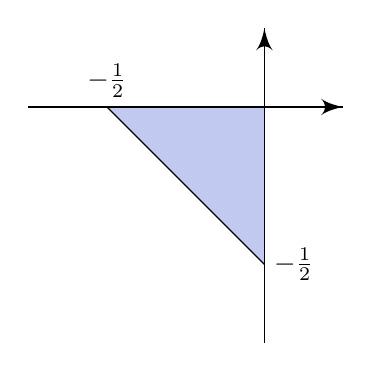
\begin{tikzpicture}
      \fill [mblue, opacity=0.3] (0, -2) -- (-2, 0) -- (0, 0);
      \draw [->] (-3, 0) -- (1, 0);
      \draw [->] (0, -3) -- (0, 1);
      \draw (-2, 0) node [above] {$-\frac{1}{2}$} -- (0, -2) node [right] {$-\frac{1}{2}$};
    \end{tikzpicture}
  \end{center}
  The three vertices are $\mu([0:0:1]), \mu([0:1:0])$ and $\mu([1:0:0])$.
\end{eg}

We now want to prove the convexity theorem. We first look at (iii). While it seems like a very strong claim, it actually follows formally from (ii).
\begin{lemma}
  (ii) implies (iii).
\end{lemma}

\begin{proof}
  Suppose the fixed point set of the action has $k$ connected components $Z = Z_1 \cup \cdots \cup Z_k$. Then $\mu$ is constant on each $Z_j$, since $X^\#|_{Z_j} = 0$ for all $X$. Let $\mu(Z_j) = \eta_j \in \R^n$. By (ii), we know the convex hull of $\{\eta_1, \ldots \eta_k\}$ is contained in $\mu(M)$.

  To see that $\mu(M)$ is exactly the convex hull, observe that if $X \in \R^n$ has rationally independent components, so that $X$ topologically generates $T$, then $p$ is fixed by $T$ iff $X_p^\# = 0$, iff $\d \mu_p^X = 0$. Thus, $\mu^X$ attains its maximum on one of the $Z_j$.

  Now if $\xi$ is not in the convex hull of $\{\eta_j\}$, then we can pick an $X \in \R^n$ with rationally independent components such that $\bra \xi, X\ket > \bra \eta_j, X\ket$ for all $j$, since the space of such $X$ is open and non-empty. Then
  \[
    \bra \xi, X\ket > \sup_{p \in \bigcup Z_j} \bra \mu(p), X\ket = \sup_{p \in M} \bra \mu(p), X\ket.
  \]
  So $\xi \not \in \mu(M)$.
\end{proof}

With a bit more work, (i) also implies (ii).
\begin{lemma}
  (i) implies (ii).
\end{lemma}
\begin{proof}
  The case $n = 1$ is immediate, since $\mu(M)$ is compact and connected, hence a closed interval.

  In general, to show that $\mu(M)$ is convex, we want to show that the intersection of $\mu(M)$ with any line is connected. In other words, if $\pi: \R^{n + 1} \to \R^n$ is any projection and $\nu = \pi \circ \mu$, then
  \[
    \pi^{-1}(c) \cap \mu(M) = \mu(\nu^{-1}(c))
  \]
  is connected. This would follow if we knew $\nu^{-1}(c)$ were connected, which would follow from (i) if $\nu$ were a moment map of an $T^n$ action. Unfortunately, most of the time, it is just the moment map of an $\R^n$ action. For it to come from a $T^n$ action, we need $\pi$ to be represented by an \emph{integer} matrix. Then
  \[
    T = \{\pi^T t : t \in T^n = \R^n /\Z^n\} \subseteq T^{n + 1}
  \]
  is a subtorus, and one readily checks that $\nu$ is the moment map for the $T$ action.

  Now for any $p_0, p_1 \in M$, we can find $p_0', p_1'$ arbitrarily close to $p_0, p_1$ and a line of the form $\pi^{-1}(c)$ with $\pi$ integral. Then the line between $p_0'$ and $p_1'$ is contained in $\mu(M)$ by the above argument, and we are done since $\mu(M)$ is compact, hence closed.
\end{proof}

It thus remains to prove (i), where we have to put in some genuine work. This requires \emph{Morse--Bott theory}.

Let $M$ be a manifold, $\dim M = m$, and $f: M \to \R$ a smooth map. Let
\[
  \Crit(f) = \{p \in M: \d f_p = 0\}
\]
be the set of critical points. For $p \in \Crit(f)$ and $(U, x_1, \ldots, x_m)$ a coordinate chart around $p$, we have a \term{Hessian matrix}
\[
  H_pf = \left( \frac{\partial^2 f}{\partial x_i \partial x_j}\right)
\]
\begin{defi}[Morse(-Bott) function]\index{Morse function}
  $f$ is a \emph{Morse function} if at each $p \in \Crit(f)$, $H_p f$ is non-degenerate.

  $f$ is a \term{Morse--Bott function} if the connected components of $\Crit(f)$ are submanifolds and for all $p \in \Crit(p)$, $T_p \Crit(f) = \ker (H_p f)$.
\end{defi}
If $f$ is Morse, then the critical points are isolated. If $f$ is Morse--Bott, then the Hessian is non-degenerate in the normal bundle to $\Crit(f)$.

If $M$ is compact, then there is a finite number of connected components of $\Crit(f)$. So we have
\[
  \Crit(f) = Z_1 \cup \cdots \cup Z_k,
\]
and the $Z_i$ are called the \term{critical submanifolds}.

For $p \in Z_i$, the Hessian $H_p f$ is a quadratic form and we can write
\[
  T_p M = E_p^- \oplus T_p Z_i \oplus E_p^+,
\]
where $E_p^{\pm}$ are the positive and negative eigenspaces of $H_p f$ respectively. Note that $\dim E_p^{\pm}$ are locally constant, hence constant along $Z_i$. So we can define the \term{index} of $Z_i$ to be $\dim E_p^-$, and the \term{coindex} to be $\dim E_p^+$.

We can then define a vector bundle $E^- \to Z_i$, called the \term{negative normal bundle}.

Morse theory tells us how the topology of $M_c^- = \{p \in M: f(p) \leq c\}$ changes with $c \in \R$.
\begin{thm}[Morse theory]\index{Morse theory}\leavevmode
  \begin{enumerate}
    \item If $f^{-1}([c_1, c_2])$ does not contain any critical point. Then $f^{-1}(c_1) \cong f^{-1}(c_2)$ and $M_{c_1} \cong M_{c_2}$ (where $\cong$ means diffeomorphic).
    \item If $f^{-1}([c_1, c_2])$ contains one critical manifold $Z$, then $M_{c_2}^- \simeq M_{c_1}^- \cup D(E^-)$, where $D(E^-)$ is the disk bundle of $E^-$.

      In particular, if $Z$ is an isolated point, $M_{c_2}^-$ is, up to homotopy equivalence, obtained by adding a $\dim E_p^-$-cell to $M_{c_1}^-$.\fakeqed
  \end{enumerate}
\end{thm}
The key lemma in this proof is the following result:
\begin{lemma}
  Let $M$ be a compact connected manifold, and $f: M \to \R$ a Morse--Bott function with no critical submanifold of index or coindex $1$. Then
  \begin{enumerate}
    \item $f$ has a unique local maximum and local minimum
    \item All level sets of $f^{-1}(c)$ are connected.
  \end{enumerate}
\end{lemma}

\begin{proof}[Proof sketch]
  There is always a global minimum since $f$ is compact. If there is another local minimum at $c$, then the disk bundle is trivial, and so in
  \[
    M_{c + \varepsilon}^- \simeq M_{c - \varepsilon}^- \cup D(E^-)
  \]
  for $\varepsilon$ small enough, the union is a disjoint union. So $M_{c + \varepsilon}$ has two components. Different connected components can only merge by crossing a level of index $1$, so this cannot happen. To handle the maxima, consider $-f$.

  More generally, the same argument shows that a change in connectedness must happen by passing through a index or coindex $1$ critical submanifold.
\end{proof}

To apply this to prove the convexity theorem, we will show that for any $X$, $\mu^X$ is a Morse--Bott function where all the critical submanifolds are symplectic. In particular, they are of even index and coindex.
\begin{lemma}
  For any $X \in \R^n$, $\mu^X$ is a Morse--Bott function where all critical submanifolds are symplectic.
\end{lemma}

\begin{proof}[Proof sketch]
  Note that $p$ is a fixed point iff $X^\#_p = 0$ iff $\d \mu^X_p = 0$ iff $p$ is a critical point. So the critical points are exactly the fixed points of $X$.

  $(T_p M, \omega_p)$ models $(M, \omega)$ in a neighbourhood of $p$ by Darboux theorem. Near a fixed point $T^n$, an equivariant version of the Darboux theorem tells us there is a coordinate chart $U$ where $(M, \omega, \mu)$ looks like
  \begin{align*}
    \omega|_U &= \sum \d x_i \wedge \d y_i\\
    \mu|_U &= \mu(p) - \frac{1}{2} \sum_i (x_i^2 + y_i^2) \alpha_i,
  \end{align*}
  where $\alpha_i \in \Z$ are \emph{weights}.

  Then the critical submanifolds of $\mu$ are given by
  \[
     \{x_i = y_i = 0 : \alpha_i \not= 0\},
  \]
  which is locally a symplectic manifold and has even index and coindex.
\end{proof}

%We now return to the proof of the convexity theorem. If $(M, \omega)$ is compact connected, $\psi: T^n \to \Symp(M, \omega)$ a Hamiltonian action with moment map $\mu: M \to \R^n$, then any $X \in \R^n$ generates a subtorus of $T^n$,
%\[
%  T^X = \{\exp tX : t \in \R\} \subseteq T^n.
%\]
%Let $f = \mu^X = \bra \mu, X\ket : M \to \R$.
%\begin{claim}
%  $\mu^X$ is a Morse--Bott function and all its critical submanifolds are symplectic and of even index and coindex.
%\end{claim}
%Then (i$_1$) is an immediate consequence of this.
%
%\begin{proof}[Proof sketch]
%  Let $p$ be a fixed point of $X$. Then $X^\#_p = 0$, and so $\d \mu^X_p = 0$, and the converse holds. So the critical points are exactly the fixed points.
%\end{proof}
Finally, we can prove the theorem.
\begin{lemma}
  (i) holds.
\end{lemma}

\begin{proof}
  The $n = 1$ case follows from the previous lemmas. We then induct on $n$.

  Suppose the theorem holds for $n$, and let $\mu = (\mu_1, \ldots, \mu_n): M \to \R^{n + 1}$ be a moment map for a Hamiltonian $T^{n + 1}$-action. We want to show that for all $c = (c_1, \ldots, c_n) \in \R^{n + 1}$, the set
  \[
    \mu^{-1}(c) = \mu_1^{-1}(c_1) \cap \cdots \cap \mu_{n + 1}^{-1}(c_{n + 1})
  \]
  is connected.

  The idea is to set
  \[
    N = \mu_1^{-1}(c_1) \cap \cdots \mu_1^{-1}(c_n),
  \]
  and then show that $\mu_{n + 1}|_N: N \to \R$ is a Morse--Bott function with no critical submanifolds of index or coindex $1$.

  We may assume that $\d \mu_1, \ldots, \d \mu_n$ are linearly independent, or equivalently, $\d \mu^X \not= 0$ for all $X \in \R^n$. Otherwise, this reduces to the case of an $n$-torus.

  To make sense of $N$, we must pick $c$ to be a regular value. Density arguments imply that
  \[
    \mathcal{C} = \bigcup_{X \not= 0} \Crit(\mu^X) = \bigcup_{X \in \Z^{n + 1} \setminus \{0\}} \Crit \mu^X.
  \]
  Since $\Crit \mu^X$ is a union of codimension $\geq 2$ submanifolds, its complement is dense. Hence by the Baire category theorem, $\mathcal{C}$ has dense complement. Then a continuity argument shows that we only have to consider the case when $c$ is a regular value of $\mu$, hence $N$ is a genuine submanifold of codimension $n$.

  By the induction hypothesis, $N$ is connected. We now show that $\mu_{n + 1}|_N: N \to \R$ is Morse--Bott with no critical submanifolds of index or coindex $1$.
%
%  By continuity, it is enough to show that $\mu^{-1}(c)$ is connected for regular values $c$. Then $N = \mu_1^{-1}(c_1) \cap \cdots \cap \mu_n^{-1}(c_n)$ is a submanifold of codimension $n$ in $M$, and by induction hypothesis, $N$ is connected. The goal is to show that
%  \[
%    \mu^{-1}(c) = N \cap \mu_{n + 1}^{-1}(c_{n + 1}) = (\mu_{n + 1}|_N)^{-1}(c_n)
%  \]
%  is connected. So we want to apply the key lemma to $\mu_{n + 1}|_N: N \to \R$. So we need to show that $\mu_{n + 1}|_N$ is Morse-Bott with no critical submanifolds of index or coindex $1$.

  Let $x$ be a critical point. Then the theory of Lagrange multipliers tells us there are some $\lambda_i \in \R$ such that
  \[
    \left[\d \mu_{n + 1} + \sum_{n = 1}^n \lambda_i \d \mu_i\right]_x = 0
  \]
  Thus, $\mu$ is critical in $M$ for the function
  \[
    \mu^Y = \mu_{n + 1} + \sum_{i = 1}^n \lambda_i \mu_i,
  \]
  where $Y = (\lambda_1, \ldots, \lambda_n, 1) \in \R^{n + 1}$. So by the claim, $\mu^Y$ is Morse--Bott with only even indices and coindices. Let $W$ be a critical submanifold of $\mu^Y$ containing $x$.
  \begin{claim}
    $W$ intersects $N$ transversely at $x$.
  \end{claim}
  If this were true, then $\mu^Y|_N$ has $W \cap N$ as a non-degenerate critical submanifold of even index and coindex, since the coindex doesn't change and $W$ is even-dimensional. Moreover, when restricted to $N$, $\sum \lambda_i \mu_i$ is a constant. So $\mu_{n + 1}|_N$ satisfies the same properties.

  To prove the claim, note that
  \[
    T_x N = \ker \d \mu_1|_x \cap \cdots \cap \ker \d \mu_n|_x.
  \]
  With a moments thought, we see that it suffices to show that $\d \mu_1, \ldots, \d \mu_n$ remain linearly independent when restricted to $T_x W$. Now observe that the Hamiltonian vector fields $X_1^\#|_x, \ldots, X_n^\#|_x$ are independent since $\d \mu_1|_x, \ldots \d \mu_n|_x$ are, and they live in $T_x W$ since their flows preserve $W$.

  Since $W$ is symplectic (by the claim), for all $k = (k_1, \ldots k_n)$, there exists $v \in T_x W$ such that
  \[
    \omega \left(\sum k_i X_i^\#|_x, v\right) \not= 0.
  \]
  In other words,
  \[
    \left(\sum k_i \d \mu_i\right)(v) \not= 0.\qedhere
  \]
\end{proof}

%\begin{proof}[Proof of (iii)]
%  Suppose the fixed point set of the action has $k$ connected components $Z = Z_1 \cup \cdots \cup Z_k$. Then $\mu$ is constant on each $Z_j$, since $X^\#|_{Z_j} = 0$ for all $X$. Let $\mu(Z_j) = \eta_j \in \R^n$.
%
%  By (ii), we know the convex hull of $\{\eta_1, \ldots \eta_k\}$ is contained in $\mu(M)$. Now suppose $\xi$ is not in the convex hull. Choose $X \in \R^n$ with rationally independent components, such that the torus topologically generated by $X$ is $T$, and such that $\bra \xi, X\ket > \bra \eta_j, X\ket$ for all $j$.
%
%  The generation condition implies that $p$ is fixed iff $X_p^\# = 0$, iff $\d \mu_p^X = 0$. This means $\mu^X$ attains its maximum on one of the $Z_j$. So
%  \[
%    \bra \xi, X\ket > \sup_{p \in M} \bra \mu(p), X\ket.
%  \]
%  So $\xi \not \in \im \mu$.
%\end{proof}

It is natural to seek a non-abelian generalization of this, and it indeed exists. Let $(M, \omega)$ be a symplectic manifold, and $G$ a compact Lie group with a Hamiltonian action on $M$ with moment map $\mu: M \to \mathfrak{g}^*$. From Lie group theory, there is a maximal torus $T \subseteq G$ with Lie algebra $\mathfrak{t}$, and the \term{Weyl group} $W = N(T)/T$ is finite (where $N(T)$ is the normalizer of $T$).

Then under the coadjoint action, we have
\[
  \mathfrak{g}^*/G \cong \mathfrak{t}^*/W,
\]
Pick a \term{Weyl chamber} $\mathfrak{t}^*_+$ of $\mathfrak{t}^*$, i.e.\ a fundamental domain of $\mathfrak{t}^*$ under $W$. Then $\mu$ induces a moment map $\mu_+: M \to \mathfrak{t}^*_+$, and the non-abelian convexity theorem says
\begin{thm}[Kirwan, 1984]
  $\mu_+(M) \subseteq \mathfrak{t}^*_+$ is a convex polytope.
\end{thm}

We shall end with an application of the convexity theorem to linear algebra. Let $\lambda = (\lambda_1, \lambda_2) \in \R^2$ and $\lambda_1 \geq \lambda_2$, and $\mathcal{H}^2_\lambda$ the set of all $2 \times 2$ Hermitian matrices with eigenvalues $(\lambda_1, \lambda_2)$. What can the diagonal entries of $A \in \mathcal{H}^2_\lambda$ be?

We can definitely solve this by brute force, since any entry in $\mathcal{H}$ looks like
\[
  A =
  \begin{pmatrix}
    a & z\\
    \bar{z} & b
  \end{pmatrix}
\]
where $a, b \in \R$ and $z \in \C$. We know
\begin{align*}
  \tr a &= a + b = \lambda_1 + \lambda_2\\
  \det a &= ab - |z|^2 = \lambda_1 \lambda_2.
\end{align*}
The first implies $b = \lambda_1 + \lambda_2 - a$, and all the second condition gives is that $ab > \lambda_1 \lambda_2$.
\begin{center}
  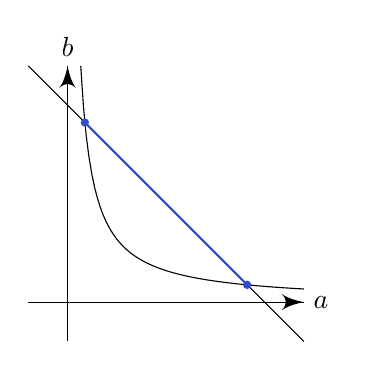
\begin{tikzpicture}
    \draw [->] (-0.5, 0) -- (3, 0) node [right] {$a$};
    \draw [->] (0, -0.5) -- (0, 3) node [above] {$b$};
    \draw [domain=0.1667:1] plot (\x, {1/(2*\x)});
    \draw [domain=1:3] plot (\x, {1/(2*\x)});

    \draw (-0.5, 3) -- (3, -0.5);

    \draw [mblue, thick] (0.2192, 2.2808) node [circ] {} -- (2.2808, 0.2192) node [circ] {};
  \end{tikzpicture}
\end{center}
This completely determines the geometry of $\mathcal{H}^2_\lambda$, since for each allowed value of $a$, there is a unique value of $b$, which in turn determines the norm of $z$. Topologically, this is a sphere, since there is a $S^1$'s worth of choices of $z$ except at the two end points $ab = \lambda_1 \lambda_2$.

What has this got to do with Hamiltonian actions? Observe that $\U(2)$ acts transitively on $\mathcal{H}_\lambda^2$ by conjugation, and
\[
  T^2 = \left\{
    \begin{pmatrix}
      e^{i\theta_1} & 0\\
      0 & e^{i\theta_2}
  \end{pmatrix}\right\} \subseteq \U(2).
\]
This contains a copy of $S^1$ given by
\[
  S^1 = \left\{
    \begin{pmatrix}
      e^{i\theta_1} & 0\\
      0 & e^{-i\theta_1}
  \end{pmatrix}\right\} \subseteq T^2.
\]
We can check that
\[
  \begin{pmatrix}
    e^{i\theta} & 0\\
    0 & e^{-i\theta}
  \end{pmatrix}
  \begin{pmatrix}
    a & z\\
    \bar{z} & b
  \end{pmatrix}
  \begin{pmatrix}
    e^{i\theta} & 0\\
    0 & e^{-i\theta}
  \end{pmatrix}^{-1} =
  \begin{pmatrix}
    a & e^{i\theta}z\\
    \overline{e^{i\theta} z} & b
  \end{pmatrix}
\]
Thus, if $\varphi: \mathcal{H}_\lambda^2 \to \R^2$ is the map that selects the diagonal elements, then
\[
  \varphi^{-1}(a, b) =
  \begin{pmatrix}
    a & |z|e^{i\theta}\\
    |z|e^{-i\theta} & b
  \end{pmatrix}\\
\]
is one $S^1$-orbit. This is reminiscent of the $S^1$ action of $S^2$ quotienting out to a line segment.

We can think more generally about $\mathcal{H}_\lambda^n$, the $n\times n$ Hermitian matrices with eigenvalues $\lambda_1 \geq \cdots \geq \lambda_n$, and ask what the diagonal elements can be.

Take $\varphi: \mathcal{H}_\lambda^n \to \R^n$ be the map that selects the diagonal entries. Then the image lies on the plane $\tr A = \sum \lambda_i$. This certainly contain the $n!$ points whose coordinates are all possible permutation of the $\lambda_i$, given by the diagonal matrices.

\begin{thm}[Schur--Horn theorem]\index{Schur--Horn theorem}
  $\varphi(\mathcal{H}_\lambda^n)$ is the convex hull of the $n!$ points from the diagonal matrices.
\end{thm}

To view this from a symplectic perspective, let $M = \mathcal{H}_\lambda^n$, and $\U(n)$ acts transitively by conjugation. For $A \subseteq M$, let $G_A$ be the stabilizer of $A$. Then
\[
  \mathcal{H}_\lambda^n = \U(n)/G_A.
\]
Thus,
\[
  T_A \mathcal{H}_\lambda^n \cong \frac{i \mathcal{H}^n}{\mathfrak{g}_A}
\]
where $\mathcal{H}^n$ is the Hermitian matrices. The point of this is to define a symplectic form. We define
\begin{align*}
  \omega_A : i \mathcal{H}^n \times i \mathcal{H}^n &\to \R\\
  (X, Y) &\mapsto i\tr([X, Y]A) = i \tr (X (YA - AY))
\end{align*}
So
\[
  \ker \omega_A = \{Y : [A, Y] = 0\} = \mathfrak{g}_A.
\]
So $\omega_A$ induces a non-degenerate form on $T_A \mathcal{H}_\lambda^n$. In fact, this gives a symplectic form on $\mathcal{H}^n_\lambda$.

Let $T^n \subseteq \U(n)$ be the maximal torus consisting of diagonal entries. We can show that the $T^n$ action is Hamiltonian with moment map $\varphi$. Since $T^n$ fixes exactly the diagonal matrices, we are done.

\subsection{Toric manifolds}
What the convexity theorem tells us is that if we have a manifold $M$ with a torus action, then the image of the moment map is a convex polytope. How much information is retained by a polytope?

Of course, if we take a torus that acts trivially on $M$, then no information is retained.

\begin{defi}[Effective action]\index{effective action}
  An action $G$ on $M$ is \emph{effective} (or \emph{faithful}) if every non-identity $g \in G$ moves at least one point of $M$.
\end{defi}

But we can still take the trivial torus $T^0$ that acts trivially, and it will still be effective. Of course, no information is retained in the polytope as well. Thus, we want to have as large of a torus action as we can. The following proposition puts a bound on ``how much'' torus action we can have:
\begin{prop}
  Let $(M, \omega)$ be a compact, connected symplectic manifold with moment map $\mu: M \to \R^n$ for a Hamiltonian $T^n$ action. If the $T^n$ action is effective, then
  \begin{enumerate}
    \item There are at least $n + 1$ fixed points.
    \item $\dim M \geq 2n$.
  \end{enumerate}
\end{prop}

We first state without proof a result that is just about smooth actions.
\begin{fact}
  An effective action of $T^n$ has orbits of dimension $n$.\fakeqed
\end{fact}
This doesn't mean all orbits are of dimension $n$. It just means \emph{some} orbit has dimension $n$.

\begin{proof}\leavevmode
  \begin{enumerate}
    \item If $\mu = (\mu_1, \ldots, \mu_n): M \to \R^n$ and $p$ is a point in an $n$-dimensional orbit, then $\{(\d \mu_i)_p\}$ are linearly independent. So $\mu(p)$ is an interior point (if $p$ is not in the interior, then there exists a direction $X$ pointing out of $\mu(M)$. So $(\d \mu^X)_p = 0$, and $\d \mu^X$ gives a non-trivial linear combination of the $\d \mu_i$'s that vanishes).

      So if there is an interior point, we know $\mu(M)$ is a non-degenerate polytope in $\R^n$. This mean it has at least $n + 1$ vertices. So there are at least $n + 1$ fixed points.
    \item Let $\mathcal{O}$ be an orbit of $p$ in $M$. Then $\mu$ is constant on $\mathcal{O}$ by invariance of $\mu$. So
      \[
        T_p \mathcal{O} \subseteq \ker (\d \mu_p) = (T_p \mathcal{O})^\omega.
      \]
      So all orbits of a Hamiltonian torus action are isotropic submanifolds. So $\dim \mathcal{O} \leq \frac{1}{2}\dim M$. So we are done.\qedhere
  \end{enumerate}
\end{proof}

In the ``optimal'' case, we have $\dim M = 2n$.
\begin{defi}[(Symplectic) toric manifold]\index{symplectic toric manifold}\index{toric manifold}
  A \emph{(symplectic) toric manifold} is a compact connected symplectic manifold $(M^{2n}, \omega)$ equipped with an effective $T^n$ action of an $n$-torus together with a choice of corresponding moment map $\mu$.
\end{defi}

\begin{eg}
  Take $(\CP^n, \omega_{FS})$, where the moment map is given by
  \[
    \mu([z_0:z_1:\cdots :z_n]) = - \frac{1}{2} \frac{(|z_1|^2, \ldots, |z_n|^2)}{|z_0|^2 + |z_1|^2 + \cdots + |z_n|^2}.
  \]
  Then this is a symplectic toric manifold.
\end{eg}

Note that if $(M, \omega, T \mu)$ is a toric manifold and $\mu = (\mu_0, \ldots, \mu_n): M \to \R^n$, then $\mu_1, \ldots, \mu_n$ are commuting integrals of motion
\[
  \{\mu_i, \mu_j\} = \omega(X_i^\#, X_j^\#) = 0.
\]
So we get an integrable system.

The punch line of the section is that there is a correspondence between toric manifolds and polytopes of a suitable kind. First, we need a suitable notion of equivalence of toric manifolds.

\begin{defi}[Equivalent toric manifolds]
  Fix a torus $T = \R^{2n}/(2\pi \Z)^n$, and fix an identification $\mathfrak{t}^* \cong \mathfrak{t} \cong \R^n$. Given two toric manifolds $(M_i, \omega_i, T, \mu_i)$ for $i = 1, 2$, We say they are
  \begin{enumerate}
    \item \emph{equivalent} if there exists a symplectomorphism $\varphi: M_1 \to M_2$ such that $\varphi(x \cdot p) = x \cdot \varphi(p)$ and $\mu_2 \circ \varphi = \mu_1$.
    \item \emph{weakly equivalent} if there exists an automorphism $\lambda: T \to T$ and $\varphi: M_1 \to M_2$ symplectomorphism such that $\varphi(x, p) = \lambda(x) \cdot \varphi(p)$.
  \end{enumerate}
\end{defi}
%Let $(M_1, \omega_1, T_1, \mu_1)$ and $(M_2, \omega_2, T_2, \mu_2)$ be toric manifolds. Then they are said to be equivalent if there is a group homomorphism $\lambda: T_1 \to T_2$ and a $\lambda$-equivariant symplectomorphism $\varphi: M_1 \to M_2$, i.e.
%\[
%  \varphi(tp) = \lambda(t) \cdot \phi(p)\text{ for all }t \in T_1, p \in M_1
%\]
%such that $\d \lambda \circ \mu_1 = \mu_2 \circ \varphi$.

We also need a notion of equivalence of polytopes. Recall that $\Aut(T) = \GL(n, \Z)$, and we can define
\begin{defi}
  \[
    \mathrm{AGL}(n, \Z) = \{x \mapsto Bx + c: B \in \GL(n, \Z), c \in \R^n\}.
  \]
\end{defi}
Finally, not all polytopes can arise from the image of a moment map. It is not hard to see that the following are some necessary properties:
\begin{defi}[Delzant polytope]\index{Delzant polytope}
  A \emph{Delzant polytope} in $\R^n$ is a compact convex polytope satisfying
  \begin{enumerate}
    \item \emph{Simplicity}: There exists exactly $n$ edges out meeting at each vertex.
    \item \emph{Rationality}: The edges meeting at each vertex $P$ are of the form $P + t u_i$ for $t \geq 0$ and $u_i \in \Z^n$.
    \item \emph{Smoothness}: For each vertex, the corresponding $u_i$'s can be chosen to be a $\Z$-basis of $\Z^n$.
  \end{enumerate}
\end{defi}
Observe that all polytopes arising as $\mu(M)$ satisfy these properties.

We can equivalently define rationality and smoothness as being the exact same conditions on the outward-pointing normals to the facets (co-dimension $1$ faces) meeting at $P$.

\begin{eg}
  In $\R$, there is any Delzant polytope is a line segment. This corresponds to the toric manifold $S^2 = \CP^1$ as before, and the length of the polytope corresponds to the volume of $\CP^1$ under $\omega$.
\end{eg}

\begin{eg}
  In $\R^2$, this is Delzant polytope:
  \begin{center}
    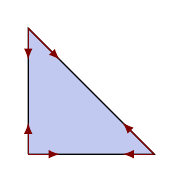
\begin{tikzpicture}[scale=0.8]
      \draw [fill=mblue, fill opacity=0.3] (0, 0) -- (0, 2) -- (2, 0) -- (0, 0);
      \draw [-latex, mred] (0, 0) -- (0.5, 0);
      \draw [-latex, mred] (0, 0) -- (0, 0.5);
      \draw [-latex, mred] (0, 2) -- (0, 1.5);
      \draw [-latex, mred] (0, 2) -- (0.5, 1.5);
      \draw [-latex, mred] (2, 0) -- (1.5, 0);
      \draw [-latex, mred] (2, 0) -- (1.5, 0.5);
    \end{tikzpicture}
  \end{center}
  On the other hand, this doesn't work:
  \begin{center}
    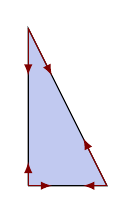
\begin{tikzpicture}
      \draw [fill=mblue, fill opacity=0.3] (0, 0) -- (1, 0) -- (0, 2) -- (0, 0);
      \draw [-latex, mred] (0, 0) -- (0.3, 0);
      \draw [-latex, mred] (0, 0) -- (0, 0.3);
      \draw [-latex, mred] (0, 2) -- (0, 1.4);
      \draw [-latex, mred] (0, 2) -- (0.3, 1.4);
      \draw [-latex, mred] (1, 0) -- (0.7, 0);
      \draw [-latex, mred] (1, 0) -- (0.7, 0.6);
    \end{tikzpicture}
  \end{center}
  since on the bottom right vertex, we have
  \[
    \det
    \begin{pmatrix}
      -1 & -1\\
      0 & 2
    \end{pmatrix} = -2 \not= \pm 1.
  \]
  To fix this, we can do
  \begin{center}
    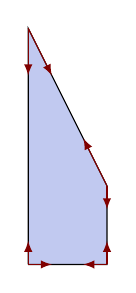
\begin{tikzpicture}
      \draw [fill=mblue, fill opacity=0.3] (0, 0) -- (0, 3) -- (1, 1) -- (1, 0) -- (0, 0);
      \draw [-latex, mred] (0, 0) -- (0.3, 0);
      \draw [-latex, mred] (0, 0) -- (0, 0.3);
      \draw [-latex, mred] (0, 3) -- (0, 2.4);
      \draw [-latex, mred] (0, 3) -- (0.3, 2.4);
      \draw [-latex, mred] (1, 1) -- (1, 0.7);
      \draw [-latex, mred] (1, 1) -- (0.7, 1.6);

      \draw [-latex, mred] (1, 0) -- (0.7, 0);
      \draw [-latex, mred] (1, 0) -- (1, 0.3);
    \end{tikzpicture}
  \end{center}
  Of course, we can also do boring things like rectangles.
\end{eg}
There is in fact a classification of all Delzant polytopes in $\R^2$, but we shall not discuss this.

\begin{eg}
  The rectangular pyramid in $\R^3$ is not Delzant because it is not simple. The tetrahedron is.
\end{eg}

\begin{thm}[Delzant]
  There are correspondences
  \begin{align*}
    \left\{\parbox{4cm}{\centering symplectic toric manifolds up to equivalence}\right\} &\longleftrightarrow \left\{\parbox{4cm}{\centering Delzant polytopes}\vphantom{\parbox{4cm}{\centering symplectic toric manifolds up to equivalence}}\right\}\\
    \left\{\parbox{4cm}{\centering symplectic toric manifolds up to weak equivalence}\right\} &\longleftrightarrow \left\{\parbox{4cm}{\centering Delzant polytopes \\modulo $\mathrm{AGL}(n, \Z)$}\vphantom{\parbox{4cm}{\centering symplectic toric manifolds up to equivalence}}\right\}
  \end{align*}
\end{thm}

\begin{proof}[Proof sketch]
  Given a Delzant polytope $\Delta$ in $(\R^n)^*$ with $d$ facets, we want to construct $(M_\Delta, \omega_\Delta, T_\Delta, \mu_\Delta)$ with $\mu_\Delta(M_\Delta) = \Delta$. The idea is to perform the construction for the ``universal'' Delzant polytope with $d$ facets, and then obtain the desired $M_\Delta$ as a symplectic reduction of this universal example. As usual, the universal example will be ``too big'' to be a genuine symplectic toric manifold. Instead, it will be non-compact.

  If $\Delta$ has $d$ facets with primitive outward-point normal vectors $v_1, \ldots, v_d$ (i.e.\ they cannot be written as a $\Z$-multiple of some other $\Z$-vector), then we can write $\Delta$ as
  \[
    \Delta = \{x \in (\R^n)^* : \bra x, v_i \ket \leq \lambda_i\text{ for }i = 1, \ldots, d\}
  \]
  for some $\lambda_i$.

  There is a natural (surjective) map $\pi: \R^d \to \R^n$ that sends the basis vector $e_d$ of $\R^d$ to $v_d$. If $\lambda = (\lambda_1, \ldots, \lambda_d)$, and we have a pullback diagram
   \[
    \begin{tikzcd}[column sep=large]
      \Delta \ar[d, hook] \ar[r] & \R^d_\lambda \ar[d, hook]\\
      (\R^n)^* \ar[r, hook, "\pi^*"] & (\R^d)^*
    \end{tikzcd}
  \]
  where
  \[
    \R^d_\lambda = \{X \in (\R^d)^* : \bra X, e_i\ket \leq \lambda_i\text{ for all }i\}.
  \]
  In more down-to-earth language, this says
  \[
    \pi^*(x) \in \R^d_\lambda \Longleftrightarrow x \in \Delta,
  \]
  which is evident from definition.

  Now there is a universal ``toric manifold'' with $\mu(M) = \R^d_\lambda$, namely $(\C^d, \omega_0)$ with the diagonal action
  \[
    (t_1, \ldots, t_d) \cdot (z_1, \ldots, z_d) = (e^{it_1} z_1, \ldots, e^{it_n}z_n),
  \]
  using the moment map
  \[
    \phi(z_1, \ldots, z_d) = -\frac{1}{2}(|z_1|^2, \ldots, |z_d|^2) + (\lambda_1, \ldots,\lambda_d).
  \]

  We now want to pull this back along $\pi^*$. To this extent, note that $\pi$ sends $\Z^d$ to $\Z^n$, hence induces a map $T^d \to T^n$ with kernel $N$. If $\mathfrak{n}$ is the Lie algebra of $N$, then we have a short exact sequence
  \[
    0 \longrightarrow (\R^n)^* \overset{\pi^*}{\longrightarrow} (\R^d)^* \overset{i^*}{\longrightarrow} \mathfrak{n}^* \longrightarrow 0.
  \]
  Since $\im \pi^* = \ker i^*$, the pullback of $\C^d$ along $\pi^*$ is exactly
  \[
    Z = (i^* \circ \phi)^{-1}(0).
  \]
  It is easy to see that this is compact.

  Observe that $i^* \circ \phi$ is exactly the moment map of the induced action by $N$. So $Z/N$ is the symplectic reduction of $\C^d$ by $N$, and in particular has a natural symplectic structure. It is natural to consider $Z/N$ instead of $Z$ itself, since $Z$ carries a $T^d$ action, but we only want to be left with a $T^n$ action. Thus, after quotienting out by $N$, the $T^d$ action becomes a $T^d/N \cong T^n$ action, with moment map given by the unique factoring of
  \[
    Z \hookrightarrow \C^d \to (\R^d)^*
  \]
  through $(\R^n)^*$. The image is exactly $\Delta$.
%  This is not difficult. The short exact sequence
%  \[
%    0 \longrightarrow N \longrightarrow T^d \longrightarrow T^n \longrightarrow 0
%  \]
%  admits a right splitting $\sigma: T^n \to T^d$, so that
%  \[
%    T^d \cong N \times \sigma(T^n).
%  \]
%  This naturally induces a splitting $(\R^d) \cong \mathfrak{n}^* \oplus (\R^n)^*$. Then the $\sigma(T^n)$ action on $Z$ descends to one on $Z/N$, with moment map given by
%  \[
%    Z \hookrightarrow \C^d \rightarrow (\R^d)^* \cong \mathfrak{n}^* \otimes (\R^n)^* \overset{\sigma^*}{\to} (\R^n)^*,
%  \]
%  whose image is exactly $\Delta$.
%
%  By assumption, $z_1, \ldots, v_d$ span $\Z^n$ over $\Z$.
%
%  Let $e_1, \ldots, e_d$ be a basis of $\R^d$. Then there is a map $T: \R^d \to \R^n$ that sends $e_i \to v_i$. Note that this maps $\Z^d$ onto $\Z^n$. This thus induces a map $T^d = \R^d/2\pi \Z^d \to T^n / 2\pi \Z^n$.
%
%  Let $N = \ker \pi$, a $(d - n)$-dimensional Lie subgroup, and $\mathfrak{n}$ the Lie algebra. We then get an exact sequences
%  \[
%    \begin{tikzcd}[row sep=tiny]
%      0 \ar[r] & N \ar[r, "i"] & T^d \ar[r, "\pi"] & T^n \ar[r] & 0\\
%      0 \ar[r] & \mathfrak{n} \ar[r, "i"] & \R^d \ar[r, "\pi"] & \R^n \ar[r] & 0\\
%      0 \ar[r] & (\R^n)^* \ar[r, "\pi^*"] & (\R^d)^* \ar[r, "i^*"] & \mathfrak{n}^* \ar[r] & 0
%    \end{tikzcd}
%  \]
%  Now consider $(\C^d, \omega_0 = -\frac{1}{2} \sum \d z_k \wedge \d \bar{z}_k)$, with the diagonal action of $T^d$ on $\C^d$ given by
%  \[
%    (t_1, \ldots, t_d) \cdot (z_1, \ldots, z_d) = (e^{it_1} z_1, \ldots, e^{it_n}z_n)
%  \]
%  which is Hamiltonian with moment map $\phi: \C^d \to (\R^d)^*$ given by
%  \[
%    \phi(z_1, \ldots, z_d) = -\frac{1}{2}(|z_1|^2, \ldots, |z_d|^2) + (\lambda_1, \ldots,\lambda_d).
%  \]
%  The action of the subgroup $N$ is Hamiltonian with moment map
%  \[
%    \begin{tikzcd}
%      \C^d \ar[r, "\phi"] & (\R^d)^* \ar[r, "i^*"] & \mathfrak{n}^*
%    \end{tikzcd}.
%  \]
%  We want to reduce it at $0$. Let
%  \begin{multline*}
%    Z = (i^* \circ \varphi)^{-1}(0) = \phi^{-1}( (i^*)^{-1}(0) \cap \im(\phi)) \\
%    = \phi^{-1}(\ker i^* \cap \im(\phi)) = \phi^{-1}(\im \pi^* \cap \im \phi).
%  \end{multline*}
%  Since $\im \pi^* \cap \im \phi$ is $n$-dimensional, we know $\dim Z = n + d$.
%  \begin{lemma}
%    Let $N$ be a $(d - n)$-dimensional subtorus of $T^d$ and $T^d \cong N \times T^n$.
%  \end{lemma}
%  \begin{lemma}
%    $\phi(Z) = \pi^*(\Delta)$
%  \end{lemma}
%  Since $\phi$ is proper, we know
%  \begin{lemma}
%    $Z$ is compact.
%  \end{lemma}
%  \begin{lemma}
%    $N$ acts freely on $Z$.
%  \end{lemma}
%  So $M_\Delta = Z/N$ is a compact connected manifold of dimension $2n$, which has a reduced symplectic form. We seek a Hamiltonian $T^n$-action with $\mu_\Delta(M_\Delta) = \Delta$.
%
%  To see this, pick a section $\sigma: T^n \to T^d$ of $0 \to N \to T^d \to T^n \to 0$. Then $\sigma(T^n)$ is a subtorus of $T^d$ of dimension $n$, and its action on $\C^d$ descends to $Z/N$ since the composition
%  \[
%    \begin{tikzcd}
%      Z \ar[r, hook, "j"] & \C^d \ar[r, "\phi"] & (\R^d)^* \cong \mathfrak{n}^* \oplus (\R^n)^* \ar[r, "\sigma^*"] & (\R^n)^*
%    \end{tikzcd}
%  \]
%  is constant along $N$-orbits. Then
%  \[
%    \mu_\Delta(M_\Delta) = (\mu_\Delta \circ \mathrm{pr})(Z) = \sigma^* \circ \phi \circ j(z) = \sigma^* \pi^* \Delta = \Delta.\qedhere
%  \]
\end{proof}

%$(M_\Delta, \omega_\Delta, T, \mu_\Delta)$ is actually K\"ahler, and this connects to the analogous theory of toric varieties in algebraic geometry.

%In fact, $\Delta$ is the orbit space of the torus action. These Delzant polytopes contain a lot of information about the manifold. % chop off corner of |_\ of CP^2 horizontally is blowup.

\section{Symplectic embeddings}
We end with a tiny chapter on symplectic embeddings, as promised in the course description.
\begin{defi}[Symplectic embedding]\index{symplectic embedding}
  A symplectic embedding is an embedding $\varphi: M_1 \hookrightarrow M_2$ such that $\varphi^* \omega_2 = \omega_1$. The notation we use is $(M_1, \omega_1) \overset{s}{\hookrightarrow} (M_2, \omega_2)$.
\end{defi}

A natural question to ask is, if we have two symplectic manifolds, is there a symplectic embedding between them?

For concreteness, take $(\C^n, \omega_0) \cong (\R^{2n}, \omega_0)$, and consider the subsets $B^{2n}(r)$ and $Z^{2n}(R) = B^2(R) \times \R^{2n - 2}$ (where the product is one of symplectic manifolds). If $r \leq R$, then there is a natural inclusion of $B^{2n}(r)$ into $Z^{2n}(R)$? If we only ask for volume-preserving embeddings, then we can always embed $B^{2n}(r)$ into $Z^{2n}(R)$, since $Z^{2n}(R)$ has infinite volume. It turns out, if we require the embedding to be symplectic, we have
\begin{thm}[Non-squeezing theorem, Gromov, 1985]\index{non-squeezing theorem}
  There is an embedding $B^{2}(n) \hookrightarrow Z^{2n}(R)$ iff $r < R$.
\end{thm}

When studying symplectic embeddings, it is natural to consider the following:
\begin{defi}[Symplectic capacity]\index{symplectic capacity}
  A \emph{symplectic capacity} is a function $c$ from the set of $2n$-dimensional manifolds to $[0, \infty]$ such that
  \begin{enumerate}
    \item Monotonicity: if $(M_1, \omega_1) \hookrightarrow (M_2, \omega_2)$, then $c(M_1, \omega_1) \leq c(M_2, \omega_2)$.
    \item Conformality: $c(M, \lambda \omega) = \lambda c(M, \omega)$.
    \item Non-triviality: $c(B^{2n}(1), \omega_0) > 0$ and $c(Z^{2n}(1), \omega_0) < \infty$.
  \end{enumerate}
  If we only have (i) and (ii), this is called a \term{generalized capacity}.
\end{defi}
Note that the volume is a generalized capacity, but not a symplectic capacity.

\begin{prop}
  The existence of a symplectic capacity is equivalent to Gromov's non-squeezing theorem.
\end{prop}

\begin{proof}
  The $\Rightarrow$ direction is clear by monotonicity and conformality. Conversely, if we know Gromov's non-squeezing theorem, we can define the \emph{Gromov width}
  \[
    W_G(M, \omega) = \sup \{\pi r^2 \mid (B^{2n}(r), \omega_0) \hookrightarrow (M, \omega)\}.
  \]
  This clearly satisfies (i) and (ii), and (iii) follows from Gromov non-squeezing. Note that Darboux's theorem says there is always an embedding of $B^{2n}(r)$ into any symplectic manifold as long as $r$ is small enough.
\end{proof}

\printindex
\end{document}
